%!TEX program = xelatex
\documentclass{beamer}
\usetheme[navigation]{UMONS}
\usepackage[utf8]{inputenc}
\usepackage[UTF8, scheme=plain]{ctex}
\usepackage{verbatim}
\usepackage{graphicx}
\usepackage{color}
\usepackage{listings}
\usepackage{amsmath}

\lstset{
    backgroundcolor=\color[rgb]{1,1,0.76},
    basicstyle=\ttfamily\tiny,                  % the size of the fonts that are used for the code
    breakatwhitespace=false,                    % sets if automatic breaks should only happen at whitespace
    breaklines=true,                            % sets automatic line breaking
    captionpos=bl,                              % sets the caption-position to bottom
    commentstyle=\color{purple} \textit,        % comment style
    deletekeywords={...},                       % if you want to delete keywords from the given language
    escapeinside={\%*}{*)},                     % if you want to add LaTeX within your code
    extendedchars=true,                         % lets you use non-ASCII characters; for 8-bits encodings only, does not work with UTF-8
    frame=tRB,                                  % adds a frame around the code
    keepspaces=true,                            % keeps spaces in text, useful for keeping indentation of code (possibly needs columns=flexible)
    keywordstyle=\color{blue}\bfseries,         % keyword style
    identifierstyle=\color{green!70!black},     % identifier style
    morekeywords={*,...},                       % if you want to add more keywords to the set
    numbers=left,                               % where to put the line-numbers; possible values are (none, left, right)
    numbersep=2pt,                              % how far the line-numbers are from the code
    numberstyle=\color{black},                  % the style that is used for the line-numbers
    stepnumber=1,                               % the step between two line-numbers. If it's 1, each line will be numbered
    rulecolor=\color{black},                    % if not set, the frame-color may be changed on line-breaks within not-black text
    showspaces=false,                           % show spaces everywhere adding particular underscores; it overrides 'showstringspaces'
    showstringspaces=true,                      % underline spaces within strings only
    showtabs=false,                             % show tabs within strings adding particular underscores
    stringstyle=\color{orange},                 % string literal style
    tabsize=2,                                  % sets default tabsize to 2 spaces
}

\title[Distributed System Series]{Distributed System : BitCoin \& BlockChain}
\author[Houmin.Wei]{\textsc{Houmin Wei}}
\institute[]{%
 Electronics Engineering \& Computer Science\\
  Peking University
  \\[2ex]
  
\includegraphics[height=4ex]{figures/PKU_red}\hspace{2em}%
  \raisebox{-1ex}{
\includegraphics[height=6ex]{figures/PKU_logo}}
}

\begin{document}
\maketitle

%\begin{frame}[allowframebreaks]
%    \frametitle{Outline}
%    \tableofcontents
%\end{frame}

%\section{Introduction}

%\subsection{Discussion}

\begin{frame}
    \frametitle{What is High Availability(HA)}
    High availability is a characteristic of a system, which aims to ensure an agreed level of operational performance, usually uptime, for a higher than normal period.

    Service Level Agreements(SLA):
    \begin{table}
        \centering
        \caption{service level agreements}
        \begin{tabular}{|c|c|c|c|c|}
            \hline
            Avaiablity \%       & Downtime Per Year & Downtime Per Month & Downtime Per Week & Downtime Per Day \\
            \hline
            90 (one nine)       &     36.5 days     &     72 hours       &    16.8 hours     &    2.4 hours     \\
            \hline
            99 (two nine)       &     3.65 days     &     7.2 hours      &    1.68 hours     &    14.4 mins     \\
            \hline
            99.9 (three nine)   &     8.76 hours    &     43.8 mins      &    10.1 mins      &    1.44 mins     \\
            \hline
            99.99 (four nine)   &     52.56 mins    &     4.38 mins      &    1.01 mins      &    8.64 secs     \\
            \hline
            99.999 (five nine)  &     5.26 mins     &     25.9 secs       &    6.05 secs     &    864.3 ms      \\
            \hline
        \end{tabular}
    \end{table}
\end{frame}

\begin{frame}
    \frametitle{HA Challenges}

\begin{itemize}
    \item Master election and restructure of cluster
    \item Protection from Split-Brain
    \item Rejoining of a failed node to the cluster
    \item Add new nodes - Scale up
    \item Prevent false Failover
    \item Protection against Race Conditions and conflicts
    \item Automatic and Transparent Application connections failover
    \item Standard Components and easy setup
\end{itemize}

\end{frame}

\begin{frame}
    \frametitle{What do Etcd, Consul, and ZooKeeper do?}

\begin{itemize}
    \item Service Registration \\
        - Host, port number, and sometimes authentication credentials, protocols, versions numbers, and/or environment details.
    \item Service Discovery \\
        - Ability for client application to query the central registry to learn of service location.
    \item Consistent and durable general-purpose K/V store across distributed system.
        \begin{itemize}
            \item Some solutions support this better than others.
            \item Based on Paxos or some derivative (i.e. Raft) algorithm to quickly converge to a consistent state.
            \item Centralized locking can be based on this K/V store.
        \end{itemize}
    \item Leader Election
        \begin{itemize}
            \item Not to be confused with leader election within the quorum of Etcd/Consul nodes. This is an implementation detail this is transparent to the user. What we are talking about here is leader election among the services that are registered against Etcd/Consul.
            \item Etcd tabled their leader election module until the API stabilizes.
        \end{itemize}
    \item Other non-standard user cases:
        \begin{itemize}
            \item Distributed locking
            \item Atomic broadcast
            \item Sequence numbers
            \item Pointers to data in eventually consistent stores.
        \end{itemize}
\end{itemize}

\end{frame}

\begin{frame}
    \frametitle{How do they behave in a distributed system?}

\begin{itemize}
    \item All of the solutions under consideration are primarily CP systems in the CAP context. That is, they favor consistency over availability. This means that all nodes have a consistent view of written data but at the expense of availability in the event that a network partitions occurs(i.e. loss of node)
    \item Some of these solutions will support "Stale Reads"
    \item Each solution can work with only one node. It is generally advised that we have one node. It is generally advised that we have one etcd/consul per VM/phiscal host. We do not want to have an etcd/consul per container!
\end{itemize}

\end{frame}

\begin{frame}
    \frametitle{Immediate problems that we are trying to solve:}
\begin{itemize}
    \item Get and set dynamic configuration across a distributed system
    \item Service Registration
        \begin{itemize}
            \item We need to spin up a track and have services make themselves visible via DNS.
            \item This would be useful primarily outside of production where we would want to regularly spin up and destroy tracks.
        \end{itemize}
    \item Service Discovery
\end{itemize}

\end{frame}

%\section{Design}

\subsection{Syncronization}

\begin{frame}
    \frametitle{Clock Syncronization}
\begin{itemize}
    \item Need for time syncronization
    \item Time syncronization techniques
    \item Lamport Clocks
    \item Vector Clocks
\end{itemize}
\end{frame}

\begin{frame}
    \frametitle{Inherent Limitations of a Distributed System}
    \begin{itemize}
        \item Absence of Global clock
        \begin{itemize}
            \item difficult to make temporal order of events.
            \item difficult to collect up-to-date information on the state of the entire system.
        \end{itemize}
        \item Absence of Shared Memory
        \begin{itemize}
            \item no up-to-date state of the entire system to any individual process as there's no shared memory.
            \item coherent view -- all observations of different process(computers) are made at the same physical time.
            \item complete view(global state) -- local views(local states) + message in transit difficult to obtain coherent global state.
        \end{itemize}
    \end{itemize}
\end{frame}

\begin{frame}
    \frametitle{Physical Clocks}
    \begin{block}{Problem}
        Sometimes we simply need the exact time, not just an ordering.
    \end{block}
    \begin{block}{Solution: Universal Coordinated Time(UTC)}
    \begin{itemize}
        \item Based on the number of transitions/sec of the cesium 133 atom.
        \item At present, the real time is taken as the average of some 50 cesium-clocks around the world.
        \item Introduces a leap second from time to time to compensate that days are getting longer.
    \end{itemize}
    \end{block}
    \begin{block}{Note}
        UTC is broadcast through short wave radio and satellite. Satellites can give an accuracy of about $\pm 0.5 ms$.
    \end{block}
\end{frame}

\begin{frame}
    \frametitle{Physical Clocks}
    \begin{block}{Problem}
        Suppose we have an distributed system with a UTC-receiver \\
        Somewhere in it => we still have to distributed its time to each machine.
    \end{block}
    \begin{block}{Basic Principle}
        \begin{itemize}
            \item Every machine has a timer that generates an interrupt H times per second.
            \item There is a clock in machine p that ticks on each timer interrupt. Denote the value of that clock by $C_p(t)$, where t is UTC time.
            \item Ideally, we have that for each machine p, $C_p(t) = t$, or in other words, $\frac{dC}{dt} = 1$.
        \end{itemize}
    \end{block}
\end{frame}

\begin{frame}
    \frametitle{Physical Clocks}
    \alert{In practice}: $1 - r \le \frac{dC}{dt} \le 1 + r$.
    \begin{figure}
        \centering
        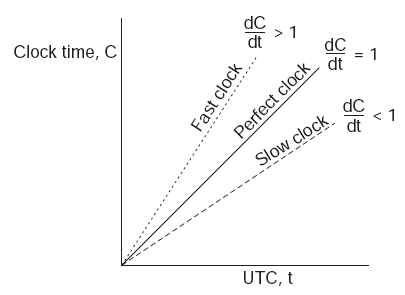
\includegraphics[scale=0.4]{phys-clock.png}
    \end{figure}
    \begin{block}{Goal}
        Never let 2 clocks in any system differ by more than $\delta$ time units => \\
        Syncronize at least every $\delta/(2r)$ seconds.
    \end{block}
\end{frame}

\begin{frame}
    \frametitle{Physical Clocks}
    Clock Syncronization Principle
    \begin{block}{Principle I}
        Every machine asks a timer server for the accurate time at least every $\delta/(2r)$ seconds(Network Time Protocol).
    \end{block}
    \begin{block}{Principle II}
        Let the server scan all machines periodically, calculate an average, and inform each machine how it should adjust its time relative to its present time.
    \end{block}
\end{frame}

\begin{frame}
    \frametitle{Logic Clock}
    \begin{block}{Why not physical clock?}
        \begin{itemize}
            \item Nodes may differ on real time at ms level using NTP.
            \item It's not necessary. If two processes do not interact, it is not necessary that their clocks be syncronized because the lack of synchronization would not be observable and thus could not cause problem.
            \item What usually matters is not that all processes agree on exactly what time it is, but rather that they agree on the order in which events occur.
        \end{itemize}
    \end{block}
\end{frame}

\begin{frame}
    \frametitle{Partial Order}
    \begin{block}{Definition}
        Orders are special binary relations. Suppose that P is a set and that $\le$ is a relation on P. Then $\le$ is a \alert{partial order} if it is \alert{reflexive}, \alert{antisymmetric}, and \alert{transitive}. i.e., for all a, b and c in P, we have that: \\
        \begin{gather}
            a \le a (reflexive) \\
            \mbox{ if } a \le b \mbox{ and } b \le a \mbox{ then } a = b (antisymmetric) \\
            \mbox{ if } a \le b \mbox{ and } b \le c \mbox{ then } a \le c (transitive)
        \end{gather}
    \end{block}
\end{frame}

\begin{frame}
    \frametitle{Happens Before}
    \begin{block}{The happens before $ a \to$ relation}
        \begin{itemize}
            \item $a \to b$, if a and b are events in the same process and a occurred before b.
            \item $a \to b$, if a is the event of sending a message m in a process and b is the event of receipt of the same message by another process
            \item if $a \to b$ and $b \to c$, then $a \to c$ (transitive).
            \item concurrent: $ a || b$ if $!(a \to b)$ and $!(b \to a)$.
            \item for any 2 events in a system, either $a \to b$ or $b \to a$ or $a || b$.
        \end{itemize}
    \end{block}
    \begin{figure}
        \centering
        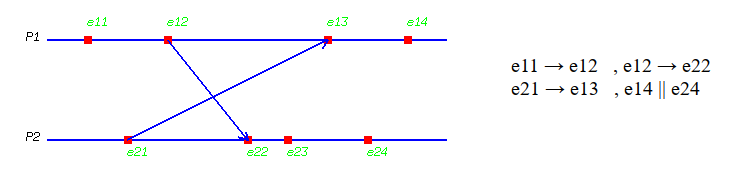
\includegraphics[scale=0.28]{lamport.png}
    \end{figure}
\end{frame}

\begin{frame}
    \frametitle{Lamport Clock}
    \begin{figure}
        \centering
        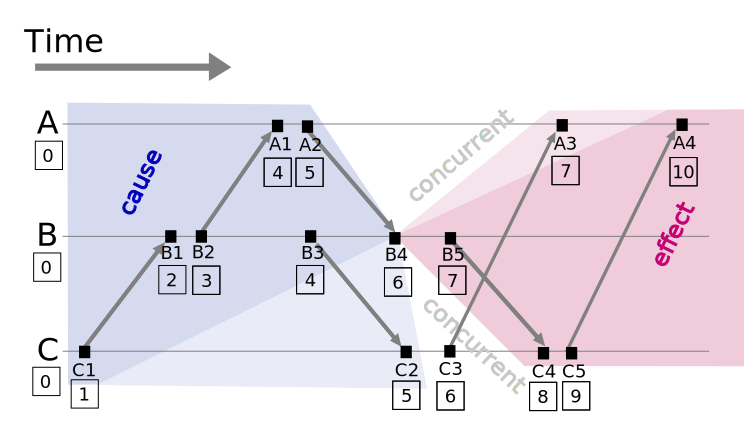
\includegraphics[scale=0.3]{Lamport-Clock}
    \end{figure}
    \begin{itemize}
        \item 每个事件对应一个Lamport时间戳,初始值为0
        \item 如果为节点内发生事件,时间戳加1
        \item 如果为发送事件,时间戳加1并在消息中带上该时间戳
        \item 如果为接收事件,时间戳=Max(本地时间戳,消息中的时间戳)+1
    \end{itemize}
\end{frame}

\begin{frame}
    \frametitle{Positioning of Lamport Clock in DS}
    \begin{figure}
        \centering
        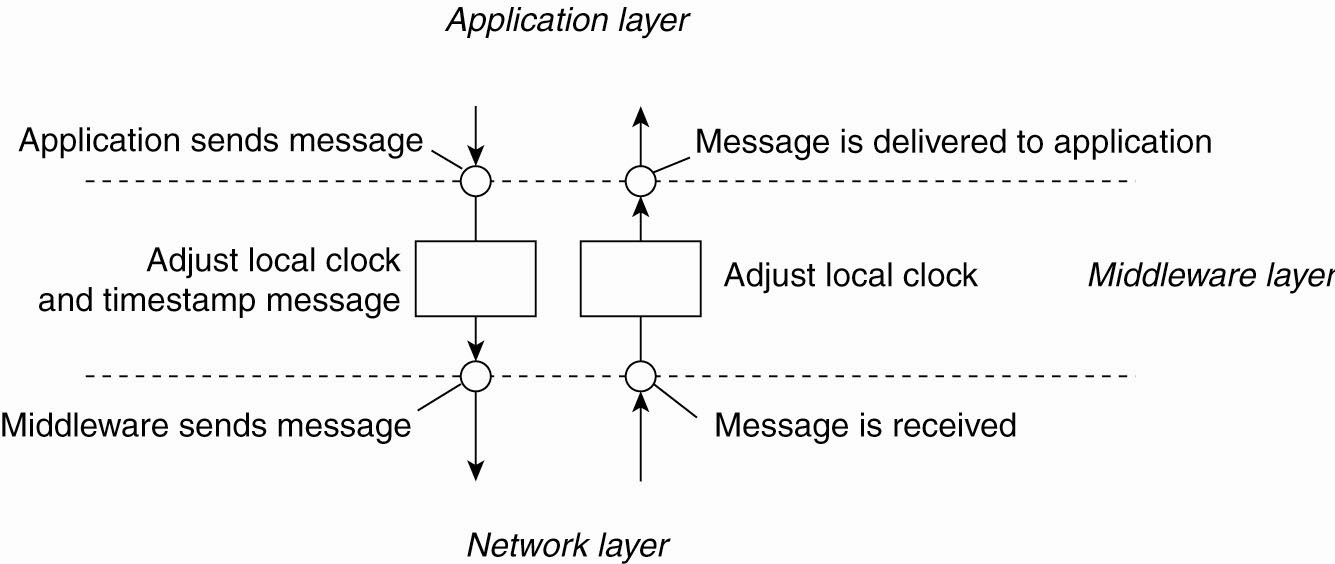
\includegraphics[scale=0.32]{lamport-position.jpg}
    \end{figure}
\end{frame}

\begin{frame}
    \frametitle{Lamport Clock}
    \begin{block}{Limitation of Lamport-Clock}
        $C_i(a)$ -- timestamp of event a at $P_i$ \\
        if $a \to b$, then $C(a) < C(b)$ \\
        but $C(a) < C(b)$ does not necessarily imply $a \to b$
    \end{block}
    \begin{itemize}
        \item Vector Clock overcome the shortcoming of Lamport Clock
        \item Goal
            \begin{itemize}
                \item Want ordering that matches causality.
                \item $C(a) < C(b)$ if and only if $a \to b$.
            \end{itemize}
        \item Method: label each event by vector V(e) [c1, c2, \ldots, cn].
    \end{itemize}
\end{frame}

\begin{frame}
    \frametitle{Vector Clock}
    \begin{figure}
        \centering
        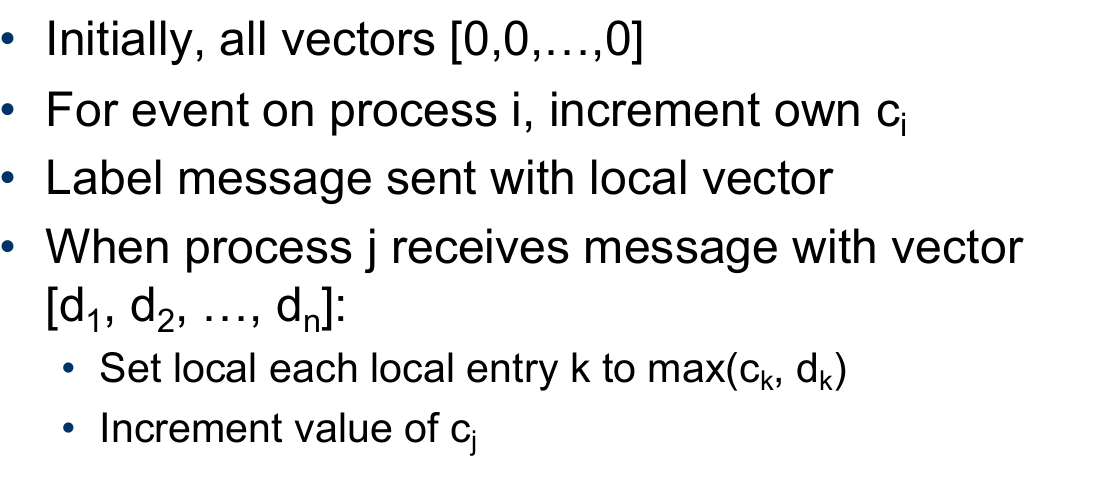
\includegraphics[scale=0.3]{vector-clock1.png}
    \end{figure}
\end{frame}

\begin{frame}
    \frametitle{Vector Clock}
    \begin{figure}
        \centering
        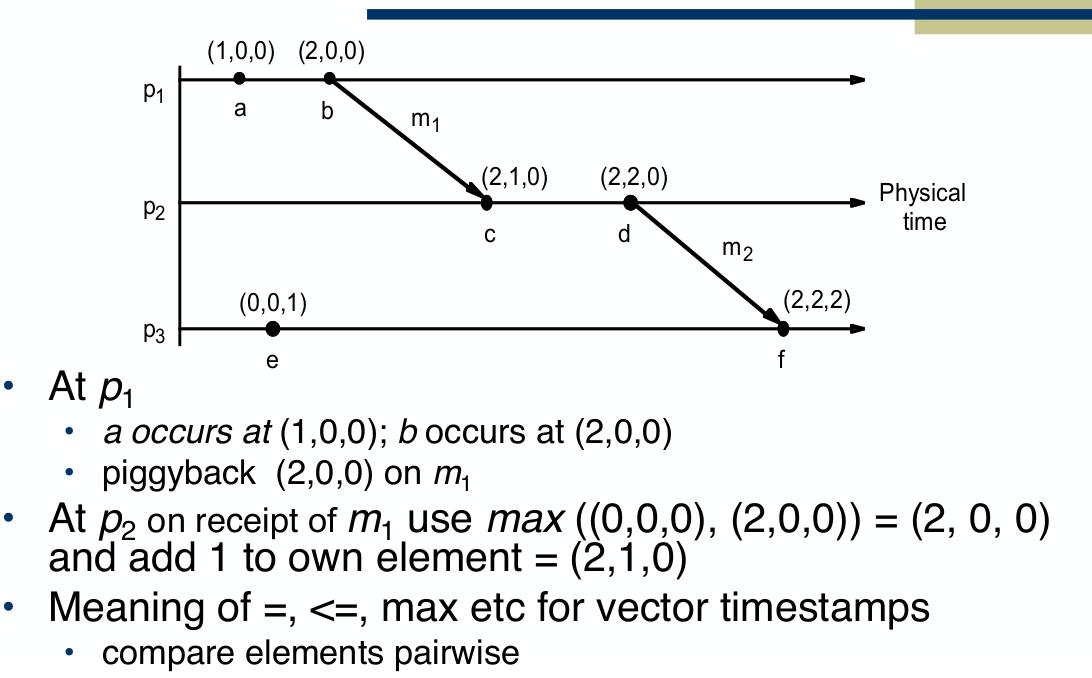
\includegraphics[scale=0.3]{vector-clock2.png}
    \end{figure}
\end{frame}

\begin{frame}
    \frametitle{Vector Clock}
    \begin{figure}
        \centering
        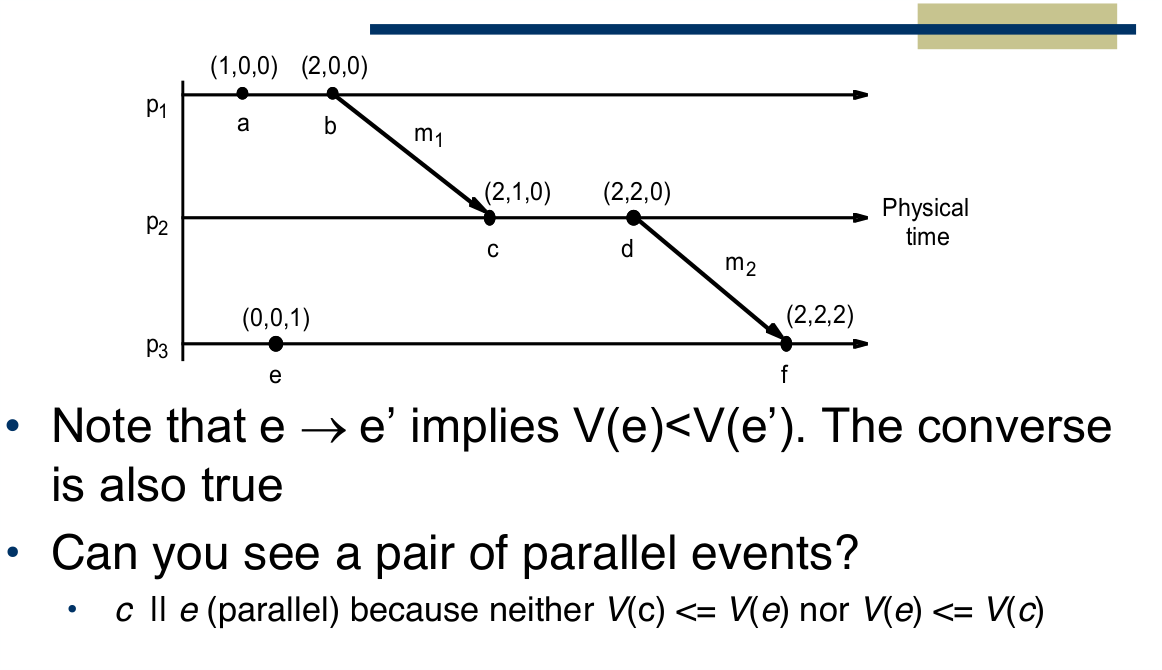
\includegraphics[scale=0.3]{vector-clock3.png}
    \end{figure}
\end{frame}

\begin{frame}
    \frametitle{Review}
    \begin{itemize}
        \item Clock Syncronization
            \begin{itemize}
                \item Rely on a time-stamped network messages
                \item Estimate delay for message transmission
                \item Can synchronize to UTC or to local source
                \item Clocks never exactly syncronized
                \item Often inadequate for distributed system
            \end{itemize}
        \item Logical Clocks
            \begin{itemize}
                \item Encode causality relationship
                \item Lamport clocks provide only one-way encoding
                \item Vector clocks provide exact causality information
            \end{itemize}
    \end{itemize}
\end{frame}

\subsection{Elections}

\begin{frame}
    \frametitle{Election Algorithms}
A Centralized Algorithm
\begin{itemize}
    \item One process is elected as the coordinator.
    \item Whenever a process wants to access a shared-resource, it sends request to the coordinator to ask for permission.
    \item Coordinator may queue requests.
\end{itemize}
\begin{figure}
    \centering
    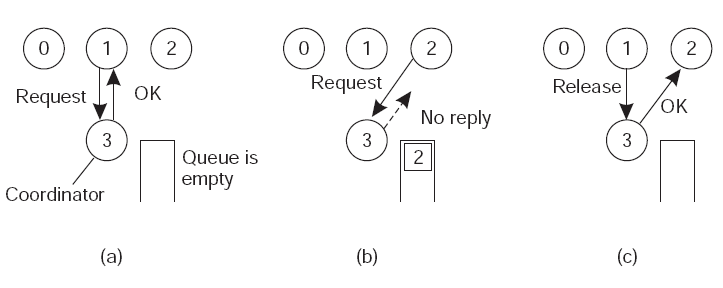
\includegraphics[scale=0.4]{mutual-exclusion.png}
\end{figure}

\end{frame}

\begin{frame}
    \frametitle{Election Algorithm}
\begin{block}{Principle}
    An algorithm requires that some process acts as a coordinator. The question is how to select this special process dynamically.
\end{block}

\end{frame}

\begin{frame}
    \frametitle{Election by bullying}
\begin{block}{Principle}
    Each process has an associated priority(weight). The process with the highest priority should always be elected as the coordinator.
\end{block}

\begin{block}{Issue: How do we find the heaviest process?}
    \begin{itemize}
        \item Any process can just start an election by sending an election message to all other processes with higher numbers.
        \item If a process $P_{heavy}$ receives an election message from a lighter process $P_{light}$, it sends a take-over message to $P_{light}$. $P_{light}$ is out of the race.
        \item If a process doesn't get a take-over message back, it wins, and sends a victory message to all other processes.
    \end{itemize}
\end{block}

\end{frame}

\begin{frame}
    \frametitle{Election by bullying}
    \begin{figure}
        \centering
        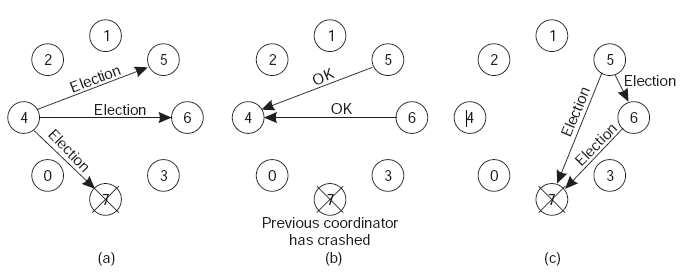
\includegraphics[scale=0.4]{bully.png}
        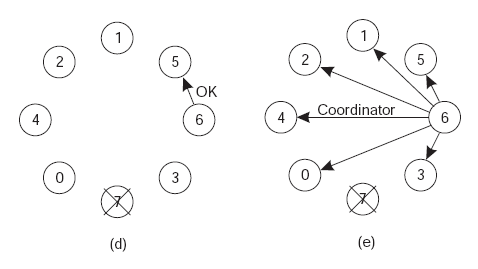
\includegraphics[scale=0.4]{bully2.png}
    \end{figure}
(a) Process 4 holds an election. \\
(b) Processes 5 and 6 responded, telling 4 to stop. \\
(c) Now 5 and 6 hold an election. \\
(d) Process 6 tells 5 to stop. \\
(e) Process 6 wins an tells everyone.
\end{frame}

\begin{frame}
    \frametitle{Election by bullying}
    \begin{block}{Issue}
    Suppose crashed nodes comes back online:
    \begin{itemize}
        \item Sends a new election message to higher numbered processes.
        \item Repeat until only one process left standing.
        \item Announces victory by sending message saying that it is coordinator(if not already coordinator)
        \item Existing(lower numbered) coordinator yields.
    \end{itemize}
    \end{block}
    Hence the term 'bully'
\end{frame}

\begin{frame}
    \frametitle{Election in a ring}
    \begin{block}{Principle}
        Process priority is obtained by organizing process into a (logical) ring. Process with the highest priority should be elected as coordinator.
    \end{block}

    \begin{itemize}
        \item Any process can start an election by sending an election message to its successor. If a successor is down, the message is passed on to the next successor.
        \item If a message is passed on, the sender adds itself to the list. When it gets back to the initiator, everyone had a chance to make its presence known.
        \item The initiator sends a coordinator message around the ring containing a list of all living processes. The one with the highest priority is elected as coordinator.
    \end{itemize}
\end{frame}


%\section{Consensus}

\begin{frame}
    \frametitle{What is Consensus?}
    \begin{itemize}
        \item Agreememt on shared state(single system image)
        \item Recovers from server failure autonomously
            \begin{itemize}
                \item Minority of servers fail: no problem
                \item Majority fail: lose availability, retain consistency
            \end{itemize}
        \begin{figure}
            \centering
            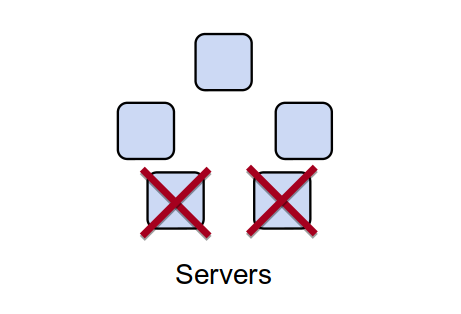
\includegraphics[scale=0.3]{concensus.png}
        \end{figure}
        \item Key to building consistent storage systems.
    \end{itemize}
\end{frame}

\begin{frame}
    \frametitle{To eliminate single point of failure: Replication}
    \begin{itemize}
        \item Network partition or server down
        \item Consensus
            \begin{itemize}
                \item Allows collection of machines to work as coherent group
                \item Continuous service, even if some machines fail
            \end{itemize}
        \item A concensus algorithm(built-in or library)
            \begin{itemize}
                \item Paxos(1990) has dominated discussion for 25 years, hard for engineer.
                \item Raft(2013) is easier to understand.
                \item \ldots
            \end{itemize}
        \item A concensus service
            \begin{itemize}
                \item Google Chubby
                \item Apache ZooKeeper
                \item \ldots
            \end{itemize}
    \end{itemize}
\end{frame}

\begin{frame}
    \frametitle{Replicated State Machine(RSM)}
    \begin{figure}
       \centering
        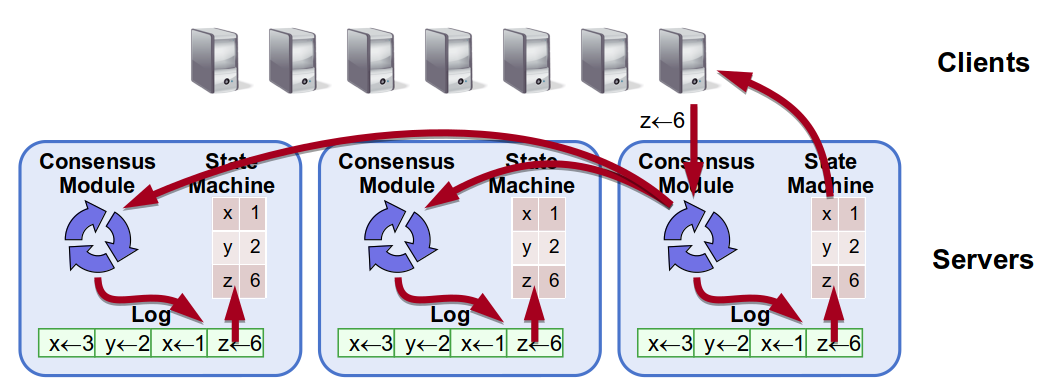
\includegraphics[scale=0.3]{rsm.png}
    \end{figure}

    \begin{itemize}
        \item Replicated log => \alert{All servers execute same commands in same order}.
        \item Consensus module ensures proper log replication.
        \item System makes progress as long as any majority of servers are up.
        \item Failure model: fail-stop(not Byzantine), delayed/lost messages.
    \end{itemize}
\end{frame}

%\subsection{Raft}

\begin{frame}
    \frametitle{Raft Overview}
    \begin{itemize}
        \item Leader election
            \begin{itemize}
                \item Select one of servers to act as cluster leader
                \item Detect crashes, choose new leader
            \end{itemize}
        \item Log replication
            \begin{itemize}
                \item Leader takes commands from clients, appends them to its log.
                \item Leader replicates its log to other servers(overwriting inconsistencies)
            \end{itemize}
        \item Safety: Only a server with an up-to-date log can become leader.
    \end{itemize}
\end{frame}

\begin{frame}
    \centering
    \href{http://thesecretlivesofdata.com/raft/}{Raft Visualization}
\end{frame}

\begin{frame}
    \frametitle{Core Raft Overview}
    \begin{itemize}
        \item Leader election
            \begin{itemize}
                \item Heartbeats and timeouts to detect crashes
                \item Randomized timeouts to avoid split votes
                \item Majority voting to guarantee at most one leader per term
            \end{itemize}
        \item Log replication
            \begin{itemize}
                \item Leader takes commands from clients, appends them to its log.
                \item Leader replicates its log to other servers(overwriting inconsistencies)
            \end{itemize}
        \item Safety
            \begin{itemize}
                \item Only elect leaders with all committed entries in their logs.
                \item New leader defers committing entries from prior terms.
            \end{itemize}
    \end{itemize}
\end{frame}

\begin{frame}
    \frametitle{Server States}
    \begin{itemize}
        \item \textbf{At any given time, each server is either:}
            \begin{itemize}
                \item \alert{Leader}: handles all client interactions, log replication
                \item \alert{Followers}: completely passive(issue no RPCs, responds to incoming RPCs)
                \item \alert{Candidate}: used to elect a new leader
            \end{itemize}
        \item \textbf{Normal operation: 1 leader, N-1 followers}
    \end{itemize}
    \begin{figure}
        \centering
        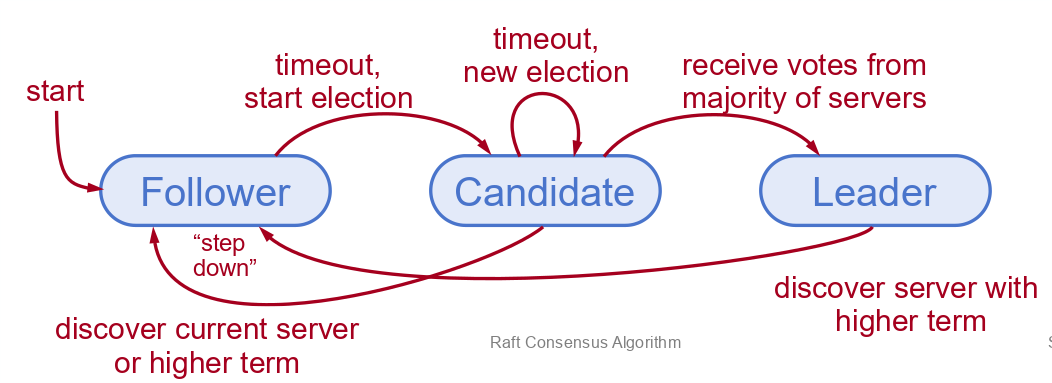
\includegraphics[scale=0.3]{raft-servers.png}
    \end{figure}
\end{frame}

\begin{frame}
    \frametitle{Terms}
    \begin{figure}
        \centering
        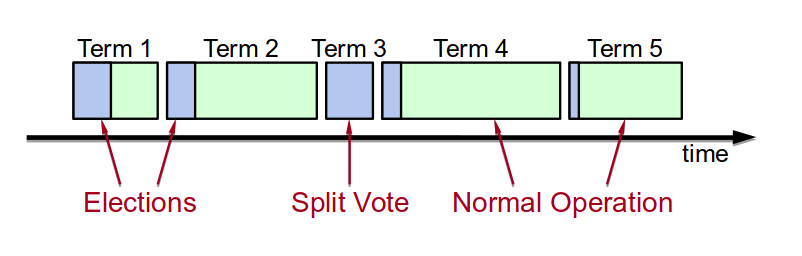
\includegraphics[scale=0.3]{raft-terms.png}
    \end{figure}
    \begin{itemize}
        \item \textbf{Time divided into terms:}
            \begin{itemize}
                \item Election
                \item Normal operation under a single leader
            \end{itemize}
        \item \textbf{At most 1 leader per term}
        \item \textbf{Some terms have no leader(failed election)}
        \item \textbf{Each server maintains \alert{current term} value}
        \item \textbf{\alert{Key role of terms: identify obsolete information}}
    \end{itemize}
\end{frame}

\begin{frame}
    \frametitle{Raft Remote Procedure Calls(RPCs)}
    \begin{itemize}
        \item \textbf{Raft servers using RPCs to communicate}
            \begin{itemize}
                \item RPC is a key piece of distribute system machinery
                \item RPC ideally make net communication look just like function call
            \end{itemize}
        \begin{figure}
            \centering
            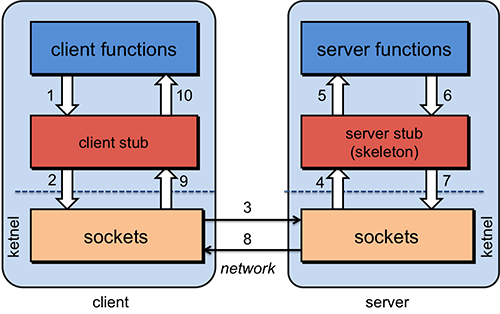
\includegraphics[scale=0.5]{rpc-flow.png}
        \end{figure}
        \item \textbf{RequestVote RPC}
            \begin{itemize}
                \item Invoked by candidate to gather votes
            \end{itemize}
        \item \textbf{AppendEntries RPC}
            \begin{itemize}
                \item Invoked by leader to replicate log entries
                \item Also used as heartbeats
            \end{itemize}
    \end{itemize}
\end{frame}

\begin{frame}
    \frametitle{RequestVote RPC}
    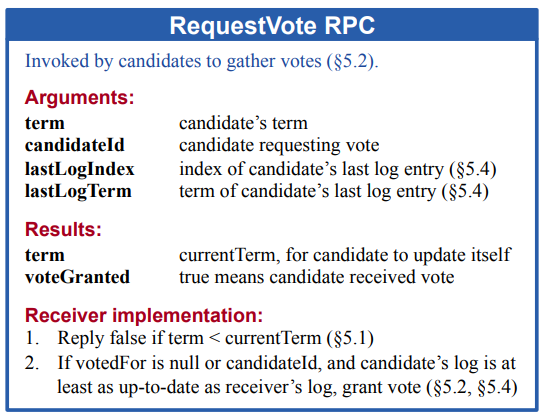
\includegraphics[scale=0.3]{raft-requestvote.png}
\end{frame}

\begin{frame}
    \frametitle{AppendEntries RPC}
    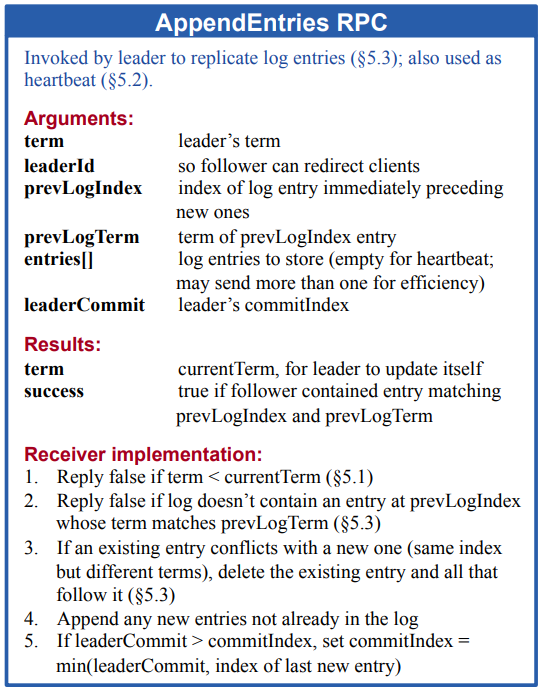
\includegraphics[scale=0.3]{raft-appendentries.png}
\end{frame}

\begin{frame}
    \frametitle{Heartbeats and Timeouts}
    \begin{itemize}
        \item \textbf{Servers start up as followers}
        \item \textbf{Followers expect to receive RPCs from leaders or candidates}
        \item \textbf{Leaders must send \alert{heartbeats}(empty AppendEntries RPCs) to maintains authority}
        \item \textbf{If \alert{election Timeout} elapses with no RPCs:}
            \begin{itemize}
                \item Follower assumes leader has crashed
                \item Follower starts new election
                \item Timeouts typically 100-500 ms
            \end{itemize}
    \end{itemize}
\end{frame}

\begin{frame}
    \frametitle{Election Basics}
    \begin{itemize}
        \item \textbf{Increment current term}
        \item \textbf{Change to Candidate state}
    \item \textbf{Vote for self}
    \item \textbf{Send RequestVote RPCs to all other servers, retry until either:}
            \begin{itemize}
                \item Receive votes from majority of servers:
                    \begin{itemize}
                        \item Become leader
                        \item Send AppendEntries heartbeats to all other servers
                    \end{itemize}
                \item Receive RPC from valid leader:
                    \begin{itemize}
                        \item Return to follower state
                    \end{itemize}
                \item No-one wins election(election timeout elapses):
                    \begin{itemize}
                        \item Increment term, start new election
                    \end{itemize}
            \end{itemize}
    \end{itemize}
\end{frame}

\begin{frame}
    \frametitle{Elections, cont'd}
    \begin{itemize}
        \item \textbf{\alert{Safety}: allow at most one winner per term}
            \begin{itemize}
                \item Each server gives out only one vote per term(persist on disk)
                \item Two different candidates can't accumulate majorities in same term
            \end{itemize}
        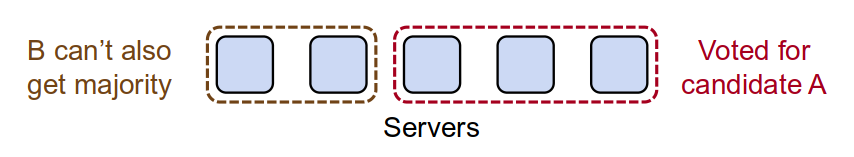
\includegraphics[scale=0.3]{raft-safety.png}
        \item \textbf{\alert{Liveness}: some candidate must eventually win}
            \begin{itemize}
                \item Choose election timeouts randomly in [T, 2T]
                \item One sever usually times out and wins election before others wake up
                \item Works well if T $\gg$ broadcast time
            \end{itemize}
    \end{itemize}
\end{frame}

\begin{frame}
    \frametitle{Log Structure}
    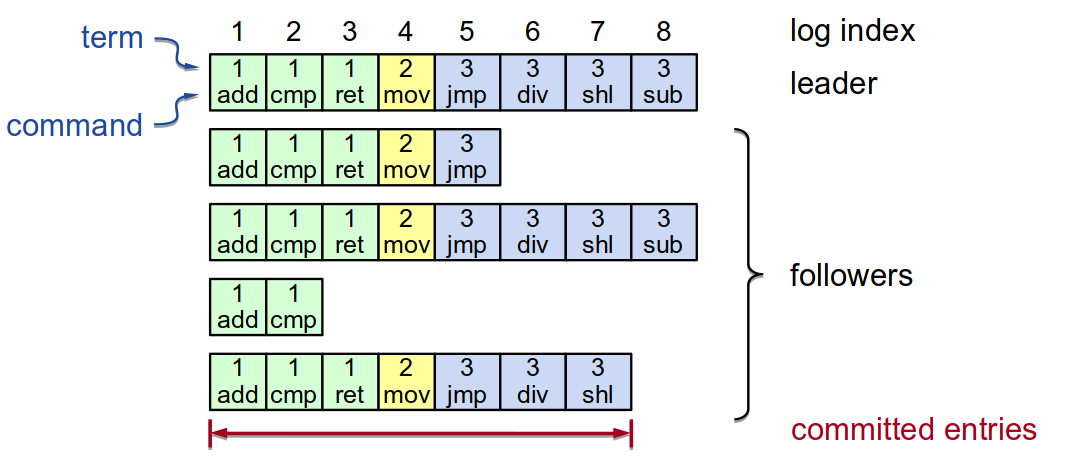
\includegraphics[scale=0.3]{raft-log.png}
    \begin{itemize}
        \item Log entry = index, term, command
        \item Log stored on stable storage(disk); survives crashes
        \item Entry \alert{committed} if known to be stored on majority of servers
            \begin{itemize}
                \item Durable, will eventually be executed by state machines
            \end{itemize}
    \end{itemize}
\end{frame}

\begin{frame}
    \frametitle{Normal Operation}
    \begin{itemize}
        \item \textbf{Client sends command to leader}
        \item \textbf{leader appends command to its log}
        \item \textbf{Leader sends AppendEntries RPCs to followers}
        \item \textbf{Once new entry committed:}
            \begin{itemize}
                \item Leader passes command to its state machine, returns result to client
                \item Leader notifies followers of committed entries in subsequent AppendEntries RPCs
                \item Followers pass committed commands to their state machines
            \end{itemize}
        \item \textbf{Crashed/slow followers?}
            \begin{itemize}
                \item Leader retries RPCs until they succeed
            \end{itemize}
        \item \textbf{Performance is optimal in common case:}
            \begin{itemize}
                \item One successful RPC to any majority of servers
            \end{itemize}
    \end{itemize}
\end{frame}

\begin{frame}
    \frametitle{Log Consistency}
    \textbf{High level of conherency between logs:}
    \begin{itemize}
        \item If log entries on different servers have same index and term:
            \begin{itemize}
                \item They store the same command
                \item The logs are identitcal in all preceding entries
            \end{itemize}
        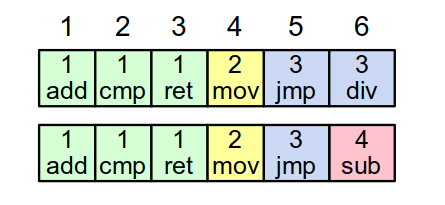
\includegraphics[scale=0.3]{raft-log2.png}
        \item If a given entry is committed, all preceding entries are also committed
    \end{itemize}
\end{frame}

\begin{frame}
    \frametitle{AppendEntries Consistency Check}
    \begin{itemize}
        \item Each AppendEntries RPC contains index, term of entry preceding new ones
        \item Follower must contain matching entry; otherwise it rejects request
        \item Implements an \alert{induction step}, ensures coherency
    \end{itemize}
    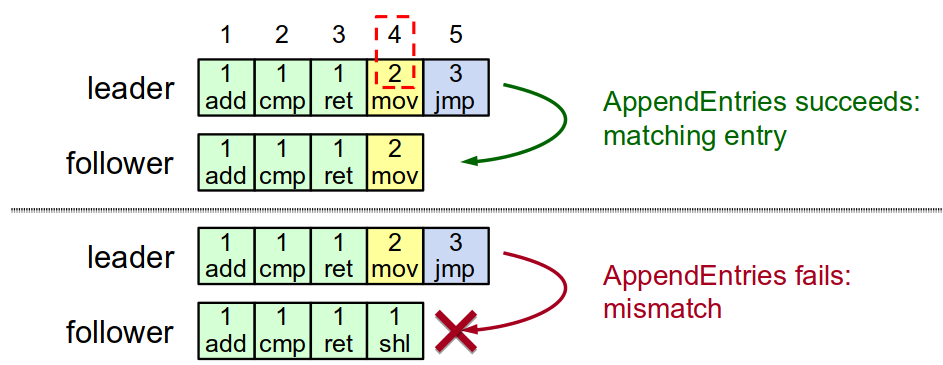
\includegraphics[scale=0.3]{raft-consistency.png}
\end{frame}

\begin{frame}
    \frametitle{Leader Changes}
    \begin{itemize}
        \item At begining of new leader's term:
            \begin{itemize}
                \item Old leader may have left entries partially replicated
                \item No special steps by new leader: just start normal operation
                \item Leader's log is \alert{the truth}
                \item Will eventually make follower's logs identical to leader's
                \item Multiple crashes can leave many extraneous log entries:
            \end{itemize}
    \end{itemize}
    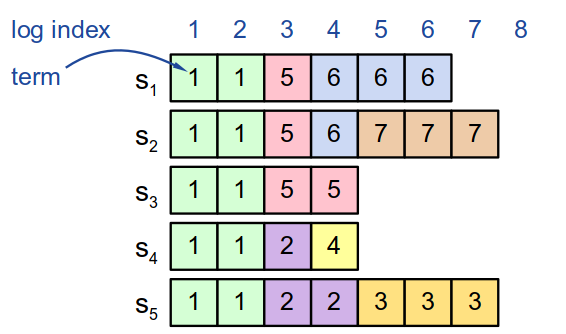
\includegraphics[scale=0.3]{raft-leader-changes.png}
\end{frame}

\begin{frame}
    \frametitle{Log Inconsistencies}
    \textbf{Leader changes can result in log inconsistencies:}
    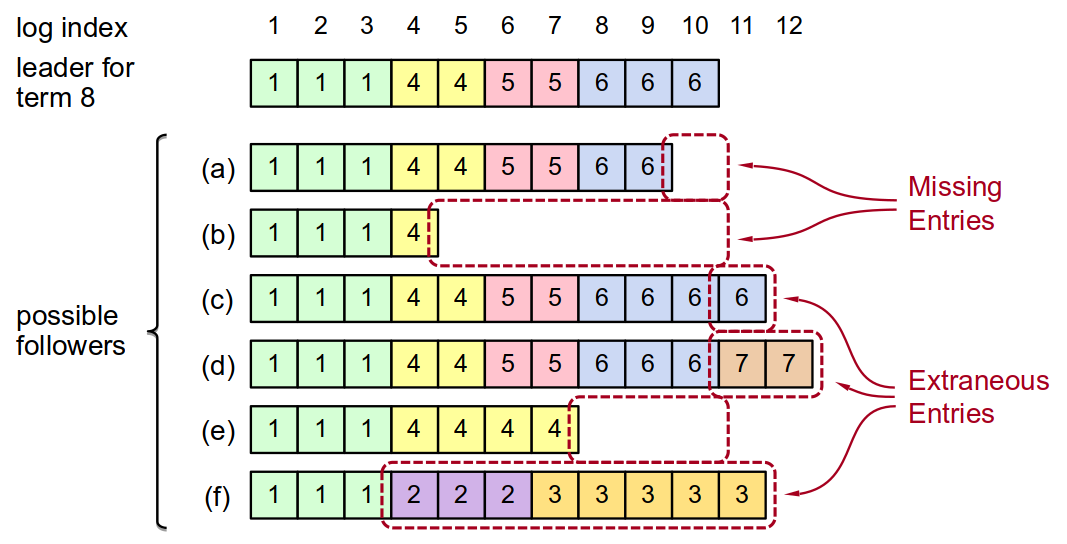
\includegraphics[scale=0.3]{raft-log-inconsistency.png}
\end{frame}

\begin{frame}
    \frametitle{Repairing Follower Logs}
    \begin{itemize}
        \item \textbf{New leader must make follower logs consistent with its own}
            \begin{itemize}
                \item Delelte extraneous entries
                \item Fill in missing entries
            \end{itemize}
        \item \textbf{Leader keeps nextIndex for each follower:}
            \begin{itemize}
                \item Index of next log entry to send to that follower
                \item Initialized to (1 + leader's last index)
            \end{itemize}
        \item \textbf{When AppendEntries Consistency Check fails, decrement nextIndex and try again:}
    \end{itemize}
    \centering
    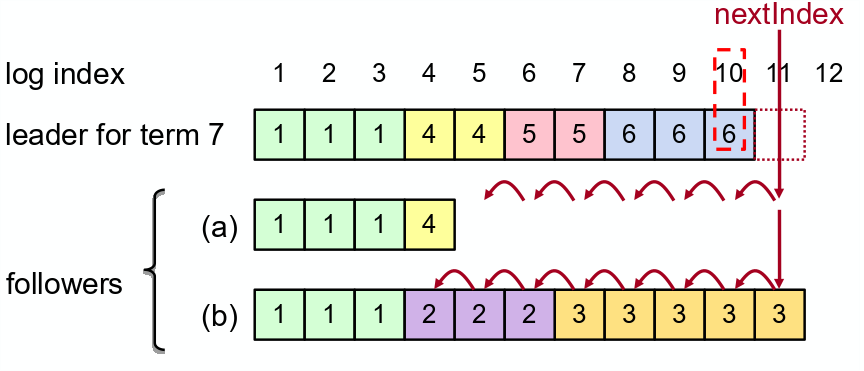
\includegraphics[scale=0.3]{raft-repairing-follower-logs.png}
\end{frame}

\begin{frame}
    \frametitle{Repairing Logs, cont'd}
    \begin{itemize}
        \item \textbf{When follower overwrites inconsistent entry, it deletes all subsequent entries:}
    \end{itemize}
    \centering
    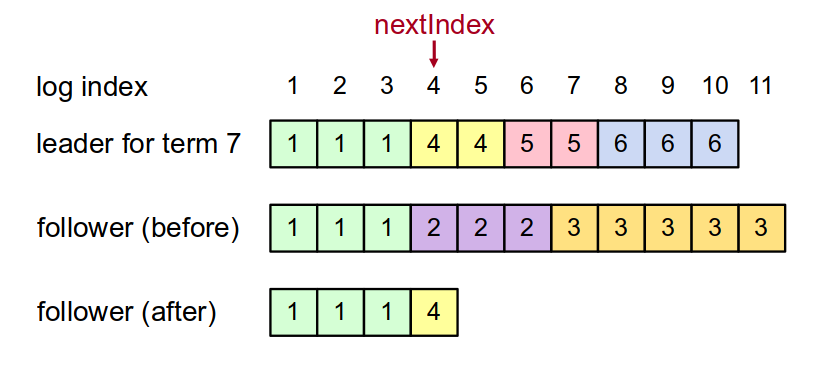
\includegraphics[scale=0.3]{raft-repariring-follower-logs2.png}
\end{frame}

\begin{frame}
    \begin{block}{Safety Requirement}
        Once a log entry has been applied to a state machine, no other state machine must apply a different value for that log entry
    \end{block}
    \begin{itemize}
        \item \textbf{Raft safety property:}
            \begin{itemize}
                \item If a leader has decided that a log entry is committed, that entry will be present in the logs of all future leaders.
            \end{itemize}
        \item \textbf{This guarantees the safety requirement}
            \begin{itemize}
                \item Leaders never overwrite entries in their logs
                \item Only entries in the leader's log can be committed
                \item Entries must be committed before applying to state machine
            \end{itemize}
    \end{itemize}
\end{frame}

\begin{frame}
    \frametitle{Picking the Best Leader}
    \begin{itemize}
        \item \textbf{Can't tell which entries are committed!}
        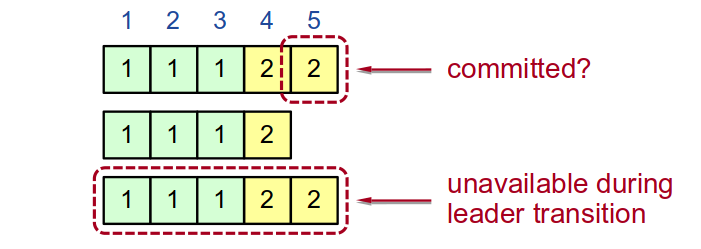
\includegraphics[scale=0.3]{raft-picking-leader.png}
        \item \textbf{During elections, choose candidate with log most likely to contain all committed entries}
            \begin{itemize}
                \item Candidates include log info in RequestVote RPCs: \\
                    (index \& term of last log entry)
                \item Voting server V denies vote if its log is 'more complete': \\
                    {\color{blue}{$(lastTerm_V > lastTerm_C) \|$}}  \\
                    {\color{blue}{$(lastTerm_V == lastTerm_C) \&\& (lastIndex_V > lastIndex_C)$}}
                \item Leader will have 'most complete' log among electing majority
            \end{itemize}
    \end{itemize}
\end{frame}

\begin{frame}
    \frametitle{Committing Entry from Current Term}
    \begin{itemize}
        \item \textbf{Case 1/2: Leader decides entry in current term is committed}
        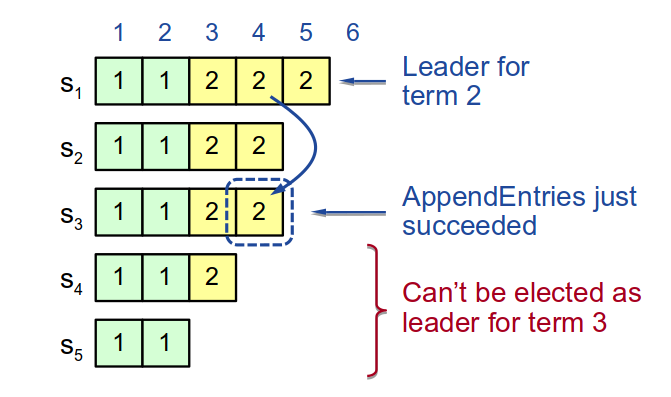
\includegraphics[scale=0.3]{raft-commit-entry.png}
        \item \textbf{Safe: leader for term 3 must contain entry 4}
    \end{itemize}
\end{frame}

\begin{frame}
    \frametitle{Committing Entry from Earlier Term}
    \begin{itemize}
        \item \textbf{Case 2/2: Leader is trying to finish committing entry from an earlier term}

        \begin{figure}
            \centering
            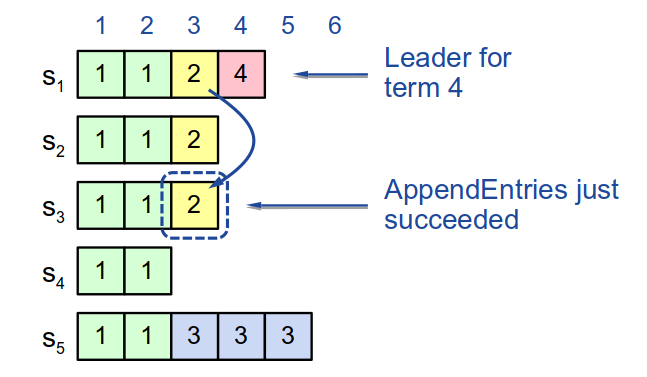
\includegraphics[scale=0.3]{raft-commite-entry2.png}
        \end{figure}

        \item \textbf{Entry 3 not safely committed:}
            \begin{itemize}
                \item $S_5$ can be elected as leader for term 5
                \item If elected, it will overwrite entry 3 on $S_1$, $S_2$, and $S_3$!
            \end{itemize}
    \end{itemize}
\end{frame}

\begin{frame}
    \frametitle{New Commitment Rules}
    \begin{minipage}{.55\textwidth}
        \begin{itemize}
            \item \textbf{For a leader to decide an entry is committed:}
                \begin{itemize}
                    \item Must be stored on a majority of servers
                    \item At least one new entry from leader's term must also be stored on majority of servers
                \end{itemize}
            \item \textbf{Once entry 4 committed:}
                \begin{itemize}
                    \item $S_5$ cannot be elected leader for term 5
                    \item Entries 3 and 4 both safe
                \end{itemize}
        \end{itemize}
    \end{minipage}
    \begin{minipage}{.4\textwidth}
        \begin{figure}[hp]
            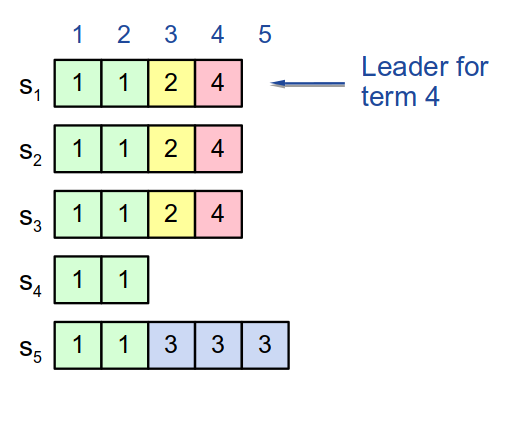
\includegraphics[scale=0.3]{raft-commit-rule.png}
        \end{figure}
    \end{minipage}
    \centering
    \textbf{Combination of election rules and Commitment rules makes Raft Safe}
\end{frame}

\begin{frame}
    \frametitle{Neutralizing Old Leaders}
    \begin{itemize}
        \item \textbf{Deposed leader may not be dead:}
            \begin{itemize}
                \item Temporarily disconnected from network
                \item Other servers elect a new leader
                \item Old leader becomes reconnected, attempts to commit log entries
            \end{itemize}
        \item \textbf{Terms used to detect stale leaders(and candidates)}
            \begin{itemize}
                \item Every RPC contains term of sender
                \item If sender's term is older, RPC is rejected, sender reverts to follower and updates its term
                \item If receiver's term is older, it reverts to follower, updates its term, then processes RPC normally
            \end{itemize}
        \item \textbf{Election updates terms of majority of servers}
            \begin{itemize}
                \item Deposed server cannot commit new log entries
            \end{itemize}
    \end{itemize}
\end{frame}

\begin{frame}
    \frametitle{Client Protocol}
    \begin{itemize}
        \item \textbf{Send commands to leader}
            \begin{itemize}
                \item If leader unknown, contact any server
                \item If contacted server not leader, it will redirected to leader
            \end{itemize}
        \item \textbf{Leader does not respond until command has been logged, committed, and executed by leader's state machine}
        \item \textbf{If request times out(e.g., leader crash)}
            \begin{itemize}
                \item Client reissues command to some other server
                \item Eventually redirected to new leader
                \item Retry request with new leader
            \end{itemize}
    \end{itemize}
\end{frame}

\begin{frame}
    \frametitle{Client Protocol, cont'd}
    \begin{itemize}
        \item \textbf{What if leader crashes after executing command, but before responding?}
            \begin{itemize}
                \item Must not execute command twice
            \end{itemize}
        \item \textbf{Solution: client embeds a unique id in each command}
            \begin{itemize}
                \item Server includes id in log entry
                \item Before accepting command, leader checks its log for entry with that id
                \item if id found in log, ignore new command, return response from old command
            \end{itemize}
        \item \textbf{Result: exactly-once semantics as long as client doesn't crash}
    \end{itemize}
\end{frame}

\begin{frame}
    \frametitle{Configuration Changes}
    \begin{itemize}
        \item \textbf{System configuration:}
            \begin{itemize}
                \item ID, address for each server
                \item Determines what constitutes a majority
            \end{itemize}
        \item \textbf{Consensus mechanism must support changes in the configuration:}
            \begin{itemize}
                \item Replace failed machine
                \item Change degree of replication
            \end{itemize}
    \end{itemize}
\end{frame}

\begin{frame}
    \frametitle{Configuration Changes, cont'd}
    \textbf{Cannot switch directly from one configuration to anther: \alert{conflicting majorities} could rise}
    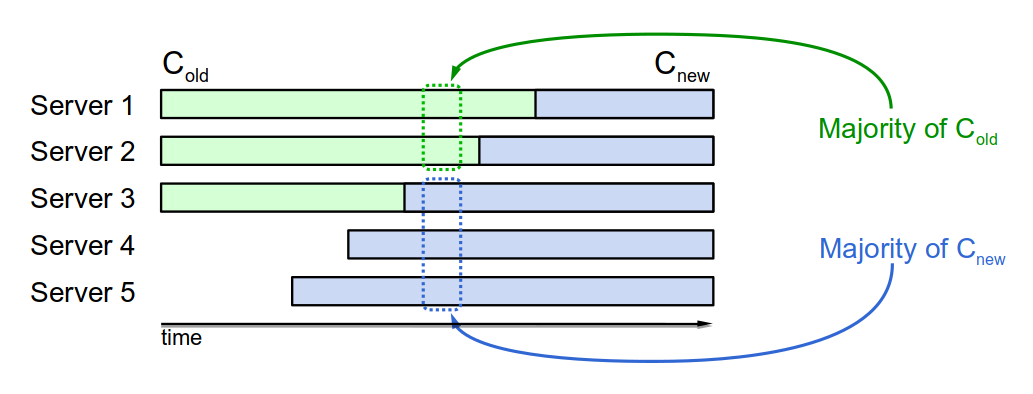
\includegraphics[scale=0.3]{raft-configuration-changes.png}
\end{frame}

\begin{frame}
    \frametitle{Joint Consensus}
    \begin{itemize}
        \item \textbf{Raft uses a 2-phase approach}
            \begin{itemize}
                \item Intermediate phase uses \alert{joint consensus}(need majority of both old and new configurations for elections, Commitment)
                \item Configuration changes is just a log entry; applied immediately on receipt(committed or not)
                \item Once joint consensus is committed, begin replicating log entry for final configuration
            \end{itemize}
    \end{itemize}
    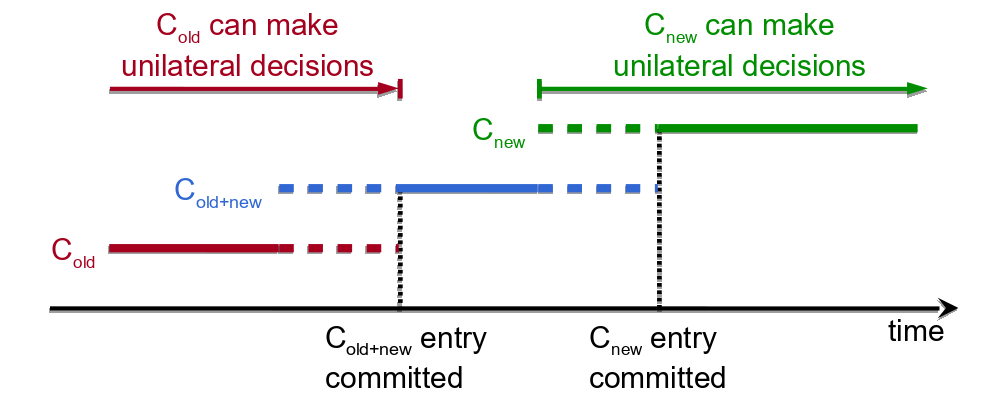
\includegraphics[scale=0.3]{raft-joint-consensus.png}
\end{frame}

\begin{frame}
    \frametitle{Joint Consensus, cont'd}
    \begin{itemize}
        \item \textbf{Additional details:}
            \begin{itemize}
                \item Any server from either configuration can serve as leader
                \item If current leader is not in $C_{new}$, must step down once $C_{new}$ is committed
            \end{itemize}
    \end{itemize}
    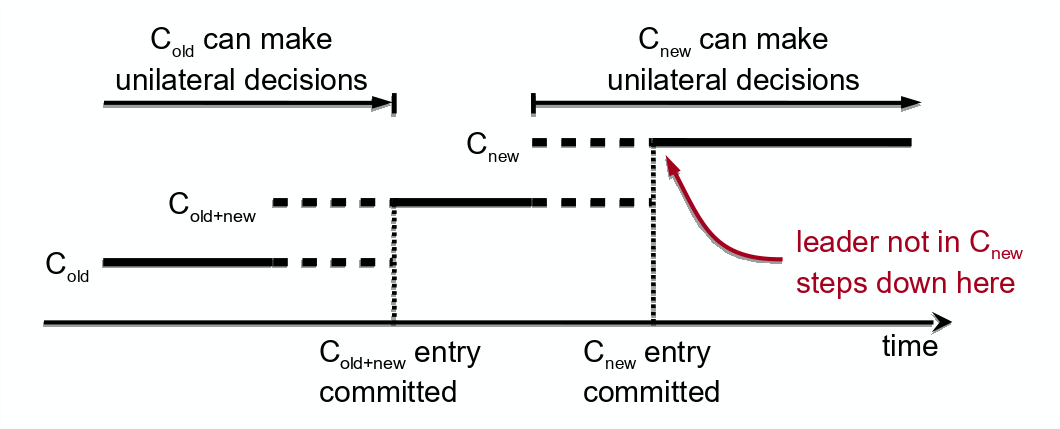
\includegraphics[scale=0.3]{raft-joint-consensus2.png}
\end{frame}




\subsection{Paxos}

\begin{frame}
    \frametitle{Paxos Algorithm}
    \begin{itemize}
        \item Leslie Lamport, 1990
        \item Nearly synonymous with consensus
    \end{itemize}
    \begin{block}{The Chubby Author}
        \emph{There is only one consensus protocol, and that's Paxos, all other approaches are just broken versions of Paxos.} \\
    \end{block}
    \begin{block}{The Chubby Author}
        \emph{There are significant gaps between the description of the Paxos algorithm and the needs of a real-world system\ldots the final system will based on an unproven protocol.}
    \end{block}
\end{frame}

%\subsection{Paxos}

\begin{frame}
    \frametitle{Paxos Algorithm}
    \begin{itemize}
        \item Leslie Lamport, 1990
        \item Nearly synonymous with consensus
    \end{itemize}
    \begin{block}{The Chubby Author}
        \emph{There is only one consensus protocol, and that's Paxos, all other approaches are just broken versions of Paxos.} \\
    \end{block}
    \begin{block}{The Chubby Author}
        \emph{There are significant gaps between the description of the Paxos algorithm and the needs of a real-world system\ldots the final system will based on an unproven protocol.}
    \end{block}
\end{frame}


%!TEX program = xelatex
\documentclass{beamer}
\usetheme[navigation]{UMONS}
\usepackage[utf8]{inputenc}
\usepackage[UTF8, scheme=plain]{ctex}
\usepackage{verbatim}
\usepackage{graphicx}
\usepackage{color}
\usepackage{listings}
\usepackage{amsmath}
\usepackage{subfigure}
\usepackage{caption}
\graphicspath{{img/}}

\lstset{
    backgroundcolor=\color[rgb]{1,1,0.76},
    basicstyle=\ttfamily\tiny,                  % the size of the fonts that are used for the code
    breakatwhitespace=false,                    % sets if automatic breaks should only happen at whitespace
    breaklines=true,                            % sets automatic line breaking
    captionpos=bl,                              % sets the caption-position to bottom
    commentstyle=\color{purple} \textit,        % comment style
    deletekeywords={...},                       % if you want to delete keywords from the given language
    escapeinside={\%*}{*)},                     % if you want to add LaTeX within your code
    extendedchars=true,                         % lets you use non-ASCII characters; for 8-bits encodings only, does not work with UTF-8
    frame=tRB,                                  % adds a frame around the code
    keepspaces=true,                            % keeps spaces in text, useful for keeping indentation of code (possibly needs columns=flexible)
    keywordstyle=\color{blue}\bfseries,         % keyword style
    identifierstyle=\color{green!70!black},     % identifier style
    morekeywords={*,...},                       % if you want to add more keywords to the set
    numbers=left,                               % where to put the line-numbers; possible values are (none, left, right)
    numbersep=2pt,                              % how far the line-numbers are from the code
    numberstyle=\color{black},                  % the style that is used for the line-numbers
    stepnumber=1,                               % the step between two line-numbers. If it's 1, each line will be numbered
    rulecolor=\color{black},                    % if not set, the frame-color may be changed on line-breaks within not-black text
    showspaces=false,                           % show spaces everywhere adding particular underscores; it overrides 'showstringspaces'
    showstringspaces=true,                      % underline spaces within strings only
    showtabs=false,                             % show tabs within strings adding particular underscores
    stringstyle=\color{orange},                 % string literal style
    tabsize=2,                                  % sets default tabsize to 2 spaces
}

\title[Distributed System Series]{Distributed System : BitCoin \& BlockChain}
\author[houmin.wei@pku.edu.cn]{\textsc{Houmin Wei}}
\institute[]{%
 Electronics Engineering \& Computer Science\\
  Peking University
  \\[2ex]
  
\includegraphics[height=4ex]{pku_red}\hspace{2em}%
  \raisebox{-1ex}{
\includegraphics[height=6ex]{pku_logo}}
}


\begin{document}
\maketitle

%\begin{frame}
%    \frametitle{Outline}
%    \tableofcontents
%\end{frame}

\section{Overview}
\begin{frame}
    \frametitle{Bitcoin Mania}
    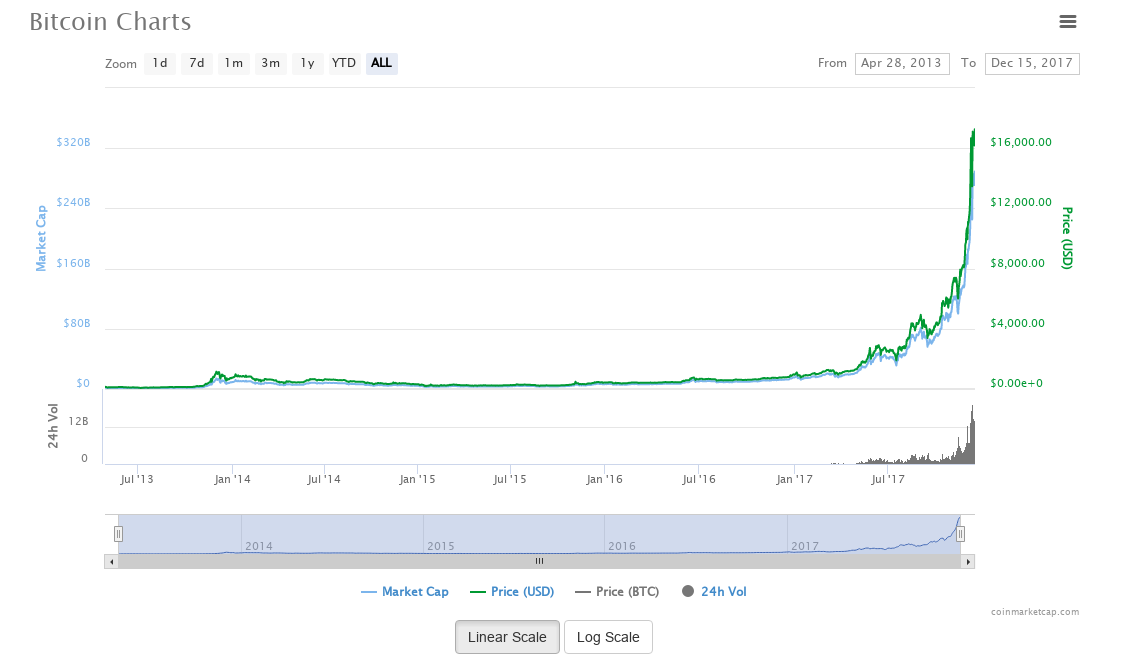
\includegraphics[scale=0.3]{bitcoin-usd-prices.png}
\end{frame}

\begin{frame}
    \frametitle{Bitcoin Mania}
    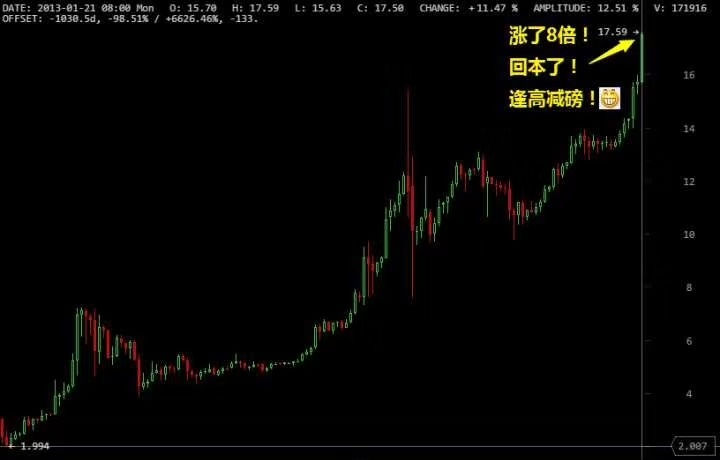
\includegraphics[scale=0.3]{bitcoin-invest0.jpg}
\end{frame}

\begin{frame}
    \frametitle{Bitcoin Mania}
    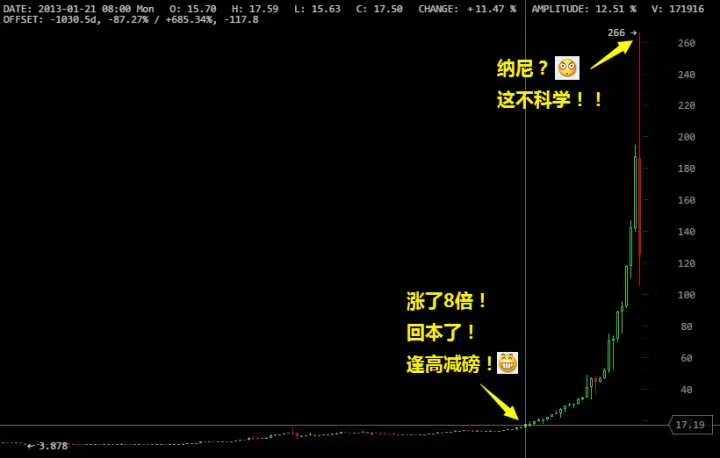
\includegraphics[scale=0.3]{bitcoin-invest1.jpg}
\end{frame}

\begin{frame}
    \frametitle{Bitcoin Mania}
    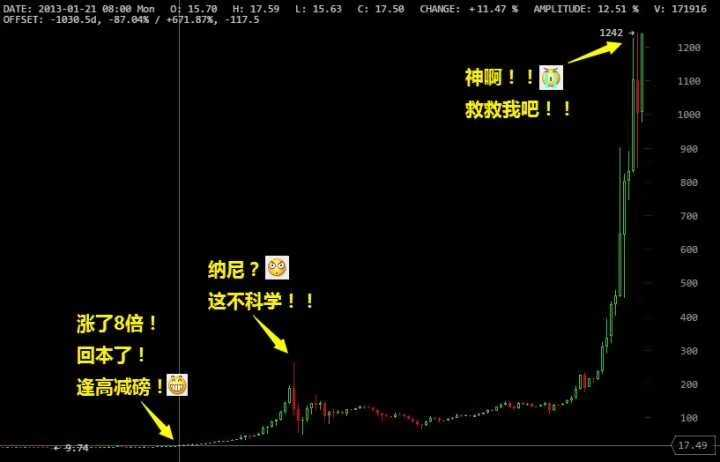
\includegraphics[scale=0.3]{bitcoin-invest2.jpg}
\end{frame}

\begin{frame}
    \frametitle{Bitcoin Mania}
    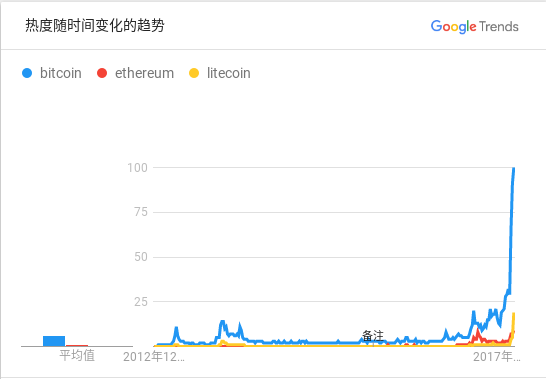
\includegraphics[scale=0.4]{bitcoin-google-trends.png}
\end{frame}

\begin{frame}
    \frametitle{Bitcoin Mania}
    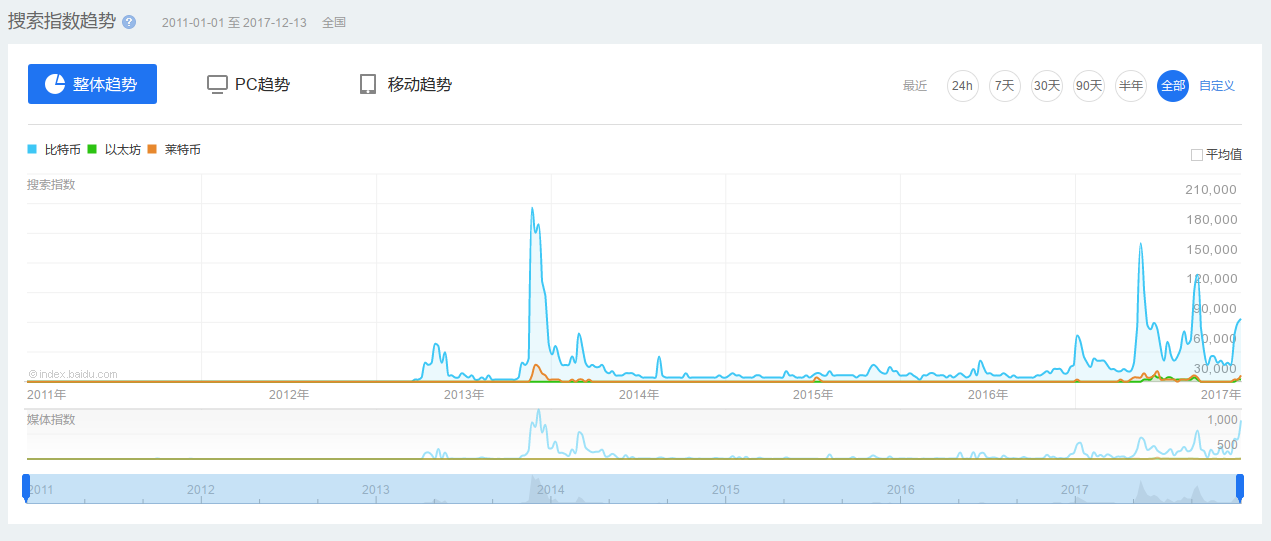
\includegraphics[scale=0.26]{bitcoin-baidu-index.png}
\end{frame}

\begin{frame}
    \frametitle{BlockChain}
    \begin{block}{国务院2016年十三五报告}
        “十三五”时期,全球信息化发展面临的环境、条件和内涵正发生深刻变化 \ldots
        信息技术创新代际周期大幅缩短,创新活力、集聚效应和应用潜能裂变式释放,更快速度、更广范围、更深程度地引发新一轮科技革命和产业变革。物联网、云计算、大数据、人工智能、机器深度学习、\alert{区块链}、生物基因工程等新技术驱动网络空间从人人互联向万物互联演进,数字化、网络化、智能化服务将无处不在。现实世界和数字世界日益交汇融合,全球治理体系面临深刻变革。全球经济体普遍把加快信息技术创新、最大程度释放数字红利,作为应对“后金融危机”时代增长不稳定性和不确定性、深化结构性改革和推动可持续发展的关键引擎。
    \end{block}
\end{frame}

\begin{frame}
    \frametitle{Barter System}
    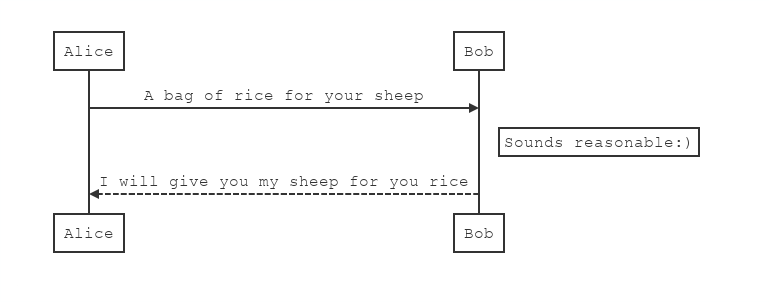
\includegraphics[scale=0.4]{barter-system.png}
\end{frame}

\begin{frame}
    \frametitle{Gold Money}
    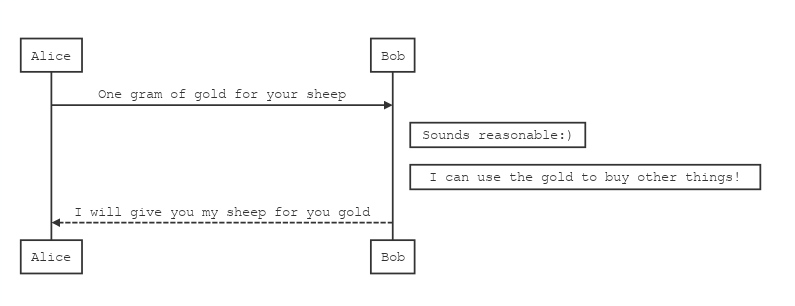
\includegraphics[scale=0.4]{gold-money.png}
\end{frame}

\begin{frame}
    \frametitle{Paper Money}
    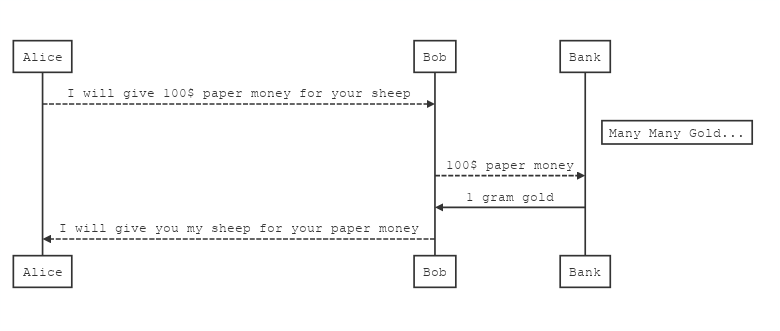
\includegraphics[scale=0.4]{paper-money.png}
\end{frame}

\begin{frame}
    \frametitle{Central Banking}
    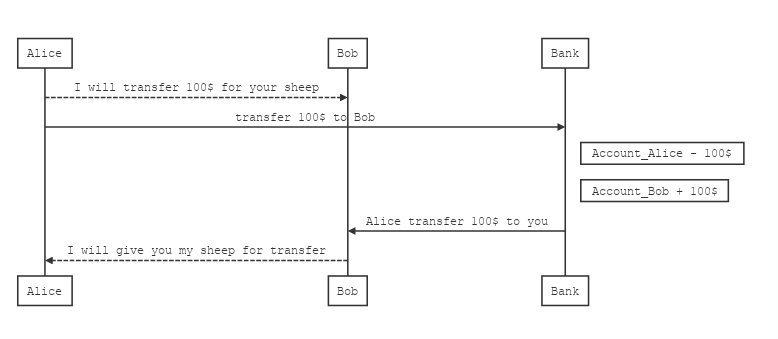
\includegraphics[scale=0.4]{central-banking.png}
\end{frame}

\begin{frame}
    \frametitle{Nature of Money}
    \textbf{What is Money?}
    \begin{itemize}
        \item \textbf{Medium of exchange}
            \begin{itemize}
                \item Standard object used in exchanging goods and services
            \end{itemize}
        \item \textbf{Unit of account}
            \begin{itemize}
                \item Standard unit used for quoting prices
            \end{itemize}
        \item \textbf{Store of value}
            \begin{itemize}
                \item Store wealth from one point in time to another
            \end{itemize}
    \end{itemize}
\end{frame}

\begin{frame}
    \frametitle{What is Bitcoin?}
    \begin{block}{Wikipedia}
        Bitcoin is the first \alert{decentralized digital cryptocurrency}, as the \alert{worldwide payment system} works without a central bank or single administrator. The network is \alert{peer-to-peer} and transactions take place between users directly through the use of cryptography, without an intermediary. These \alert{transactions} are verified by network nodes, which called \alert{mining} and recorded in a \alert{public distributed ledger} called a \alert{blockchain}. Bitcoin was invented by an unknown person or group of people under the name \alert{Satoshi Nakamoto} and released as \alert{open-source software} in 2009.
    \end{block}
\end{frame}

\begin{frame}
    \frametitle{Video}
    \begin{center}
        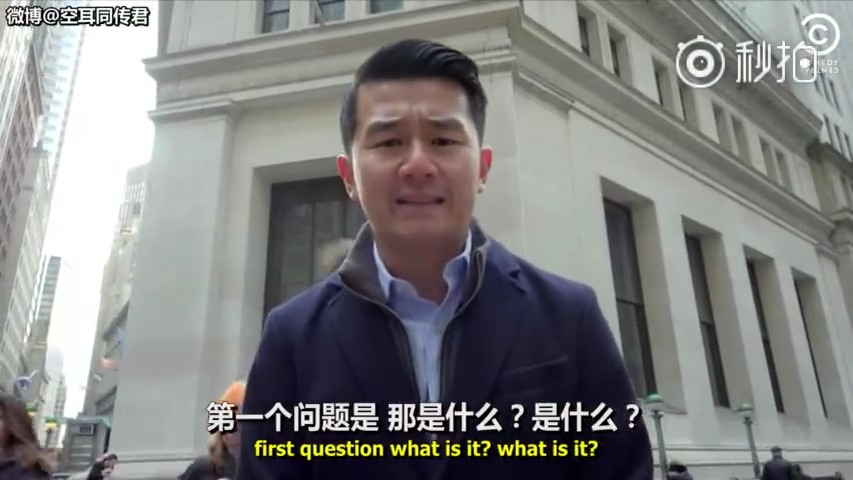
\includegraphics[scale=0.35]{what-it-it.jpg} \\
        \href{run:cryptocurrency.mp4}{\textbf{Bitcoin, What is it?}}
    \end{center}
\end{frame}

\begin{frame}
    \frametitle{Bitcoin Overview}
    
\includegraphics[scale=1]{mbc2_0201.png}
\end{frame}

\begin{frame}[fragile]
    \frametitle{Buying a cup of coffee}
    Alice buyes a cup of coffee at Bob's coffee shop, paying with BTC.
    \begin{columns}
        \begin{column}{0.6\textwidth}
            \begin{lstlisting}[language=Python]
bitcoin:1GdK9UzpHBzqzX2A9JFP3Di4weBwqgmoQA?\
amount=0.015&\
label=Bob%27s%20Cafe&\
message=Purchase%20at%20Bob%27s%20Cafe

Components of the URL
A bitcoin address: "1GdK9UzpHBzqzX2A9JFP3Di4weBwqgmoQA"
The payment amount: "0.015"
A label for the recipient address: "Bob's Cafe"
A description for the payment: "Purchase at Bob's Cafe"
            \end{lstlisting}
        \end{column}
        \begin{column}{0.3\textwidth}
            
\includegraphics[scale=1]{mbc2_0202.png}
        \end{column}
    \end{columns}
\end{frame}

\begin{frame}
    \begin{center}
        \textbf{\alert{\huge{Q \& A}}}
    \end{center}
\end{frame}

\begin{frame}
    \frametitle{Bitcoin: Challenges}
    \begin{itemize}
        \item \textbf{Creation of a virtual coin}
            \begin{itemize}
                \item How is it created in the first place?
                \item How do you prevent inflation?
            \end{itemize}
        \item \textbf{Validation}
            \begin{itemize}
                \item Is the coin legit? \alert{(Proof-Of-Work)}
                \item How do you prevent a coin from \alert{double-spending}?
            \end{itemize}
        \item \textbf{Buyer and seller protection in online transactions}
            \begin{itemize}
                \item Buyer pays, but the seller doesn't deliver
                \item Seller delivers, buyer pays, but the buyer makes a claim
            \end{itemize}
        \item \textbf{Trust on third party}
            \begin{itemize}
                \item Rely on proof instead of trust
                \item Verifiable by everyone
                \item No central bank
            \end{itemize}
    \end{itemize}
\end{frame}

\begin{frame}
    \frametitle{CryptoCurrency}
    
\includegraphics[scale=0.16]{cryptocurrency.png}
\end{frame}

\begin{frame}[fragile]
    \frametitle{Bitcoin Overview}
    \begin{lstlisting}[language=JavaScript]
function mine()
{
    while (true)
    {
        longestChain = getLongestValidChain();

         A number that changes every time, so that you don't waste time
         trying to calculate a valid blockHash with the same input.
        nonce = getNewNonce();

        currentTXs = getUnconfirmedTransactionsFromNetwork();
        newBlock = getNewBlock(longestChain, currentTX, nonce);

         Hash function, and this is what all the *mining machines* are doing
        blockHash = sha256(newBlock)

        if (meetRequirements(blockHash))
        {
            broadcast(newBlock)
             now the height of the block chain is incremented by 1
             if the new block is accepted by other peers
             and all the TXs in the new block are "confirmed"
        }
    }
}
    \end{lstlisting}
\end{frame}

\begin{frame}[fragile]
    \frametitle{Bitcoin Overview}
    \begin{lstlisting}[language=JavaScript]
function sendBTC(amount)
{
    sourceTXs = pickConfirmedTransactionsToBeSpent(amount);
    tx = generateTX(sourceTx, targetAddrs, amount, fee);
    signedTx = sign(tx, privateKeysOfAllInputAddress);
    broadcast(signedTx);
}
    \end{lstlisting}
\end{frame}



\section{P2P Network}
\begin{frame}
    \frametitle{P2P Network}
    The steps to run the network are as follows:
    \begin{itemize}
        \item New transactions are broadcast to all nodes.
        \item Each node collects new transactions into a block.
        \item When node finds a proof-of-work, it broadcast the block to all nodes.
        \item Nodes accept the block only if all transactions in it are valid and not already spent.
        \item Nodes express their acceptance of the block by working on creating the next block in the chain, using the hash of the accepted block as previous hash.
    \end{itemize}
\end{frame}

\begin{frame}
    \includegraphics[scale=0.6]{./figures/mbc2_0802.png}
\end{frame}

\begin{frame}
    \includegraphics[scale=0.15]{./figures/mbc2_0803.png}
\end{frame}


\section{Crypto}
\begin{frame}
    \frametitle{Security in Bitcoin}
    \begin{itemize}
        \item \textbf{Authentication}
            \begin{itemize}
                \item Am I paying the right person?
            \end{itemize}
        \item \textbf{Integrity}
            \begin{itemize}
                \item Is the coin double-spent?
                \item Can an attacker reverse or change transactions?
            \end{itemize}
        \item \textbf{Availability}
            \begin{itemize}
                \item Can I make a transactions anytime I want?
            \end{itemize}
        \item \textbf{Confidentiality}
            \begin{itemize}
                \item Are my transactions private? Anonymous?
            \end{itemize}
    \end{itemize}
\end{frame}

\begin{frame}
    \frametitle{Security in Bitcoin}
    \begin{itemize}
        \item \textbf{Authentication -> \alert{Public Key Crypto: Digital Signatures}}
            \begin{itemize}
                \item Am I paying the right person?
            \end{itemize}
        \item \textbf{Integrity -> \alert{Digital Signatures and Cryptographic Hash}}
            \begin{itemize}
                \item Is the coin double-spent?
                \item Can an attacker reverse or change transactions?
            \end{itemize}
        \item \textbf{Availability -> \alert{Broadcast messages to the P2P network}}
            \begin{itemize}
                \item Can I make a transactions anytime I want?
            \end{itemize}
        \item \textbf{Confidentiality -> \alert{Pesudonymity}}
            \begin{itemize}
                \item Are my transactions private? Anonymous?
            \end{itemize}
    \end{itemize}
\end{frame}

\begin{frame}
    \frametitle{Cryptographic Hash Function}
    \begin{itemize}
        \item \textbf{Computationally efficient}
        \item \textbf{Consistent} \\
            hash(x) always yields same result.
        \item \textbf{Collision Resistant} \\
            Given $hash(W) = Z$, hard to find X such that $hash(X) = Z$
        \item \textbf{One-way} \\
            Given Y, hard to find X s.t. $hash(X) = Y$
    \end{itemize}
    \begin{columns}
        \begin{column}{0.5\textwidth}
            \includegraphics[scale=0.3]{hash_functions.jpg}
        \end{column}
        \begin{column}{0.5\textwidth}
            Common Hash Functions:
            \begin{itemize}
                \item \textbf{MD5}
                \item \textbf{SHA-1}
                \item \textbf{SHA-2}
                    \begin{itemize}
                        \item SHA-256
                        \item SHA-384
                        \item SHA-512
                    \end{itemize}
            \end{itemize}
        \end{column}
    \end{columns}
\end{frame}

\begin{frame}[fragile]
    \frametitle{Hash Function Example}
    \begin{lstlisting}[language=Python]
    SHA224("")
    0x d14a028c2a3a2bc9476102bb288234c415a2b01f828ea62ac5b3e42f
    SHA256("")
    0x e3b0c44298fc1c149afbf4c8996fb92427ae41e4649b934ca495991b7852b855
    \end{lstlisting}

    Even a small change in the message wil result in a mostly different hash.
    \begin{lstlisting}[language=Python]
    SHA224("The quick brown fox jumps over the lazy dog")
    0x 730e109bd7a8a32b1cb9d9a09aa2325d2430587ddbc0c38bad911525
    SHA224("The quick brown fox jumps over the lazy dog.")
    0x 619cba8e8e05826e9b8c519c0a5c68f4fb653e8a3d8aa04bb2c8cd4c
    \end{lstlisting}

    Proof of work first sight:

    Given a basic string \alert{hello world!} + random number \alert{nonce}

    We need the digest have 4 leading 0.
    \begin{lstlisting}[language=Python]
    "Hello, world!0" => 1312af178c253f84028d480a6adc1e25e81caa44c749ec81976192e2ec934c64
    "Hello, world!1" => e9afc424b79e4f6ab42d99c81156d3a17228d6e1eef4139be78e948a9332a7d8
    "Hello, world!2" => ae37343a357a8297591625e7134cbea22f5928be8ca2a32aa475cf05fd4266b7
    ...
    "Hello, world!4248" => 6e110d98b388e77e9c6f042ac6b497cec46660deef75a55ebc7cfdf65cc0b965
    "Hello, world!4249" => c004190b822f1669cac8dc37e761cb73652e7832fb814565702245cf26ebb9e6
    "Hello, world!4250" => 0000c3af42fc31103f1fdc0151fa747ff87349a4714df7cc52ea464e12dcd4e9
    \end{lstlisting}
\end{frame}

\begin{frame}
    \frametitle{Public Key Crypto: Encryption}
    Key pair: Public Key and Private Key
    \begin{columns}
        \begin{column}{0.35\textwidth}
            \begin{center}
                \includegraphics[scale=0.1]{Public-key-crypto.png}
            \end{center}
        \end{column}
        \begin{column}{0.65\textwidth}
            \begin{center}
                \includegraphics[scale=0.1]{Public_key_shared_secret.png}
            \end{center}
        \end{column}
    \end{columns}
\end{frame}

\begin{frame}
    \frametitle{Public Key Crypto: Digital Signature}
    \includegraphics[scale=0.3]{digital-signatures-methodology.jpg}
\end{frame}

\begin{frame}
    \frametitle{Public Key to Bitcoin Address}
    \includegraphics[scale=0.5]{mbc2_0405.png}
\end{frame}



\section{Transaction}
\begin{frame}

\end{frame}


\section{BlockChain}
\begin{frame}
    \frametitle{BlockChain Overview}
    \begin{itemize}
        \item The block chain provides Bitcoin's public ledger, an ordered and timestamped record of transctions.
        \item This system is used to protect against double spending and modification of previous transactions records.
        \item Each full node in the Bitcoin network independently stores a block chain containing only blocks validated by that node.
    \end{itemize}
    \includegraphics[scale=0.4]{./figures/en-blockchain-overview.png}
\end{frame}

\begin{frame}[fragile]
    \frametitle{BlockChain Data Structure}
    \begin{columns}
        \begin{column}{0.6\textwidth}
            \includegraphics[scale=0.5]{./figures/blockchain-data-structure.png}
        \end{column}
        \begin{column}{0.4\textwidth}
            \includegraphics[scale=0.4]{./figures/mbc2_0902.png}
        \end{column}
    \end{columns}
    \begin{itemize}
        \item \textbf{Block Header}: 80 bytes, whereas transctions is at least 250 bytes.
        \item \textbf{Nonce}: A counter used for proof-of-work algorithm.
        \item \textbf{Difficulty}: How difficult it is to find a hash below a given target.
        \item \textbf{Coinbase}: The content of the \alert{input} of a generation transction.
    \end{itemize}
    \begin{lstlisting}[language=Python]
The Times 03/Jan/2009 Chancellor on brink of second bailout for banks. \end{lstlisting}
\end{frame}

\begin{frame}[fragile]
    \frametitle{The Genesis Block}
    \begin{lstlisting}[language=Python]
bitcoind getblock 000000000019d6689c085ae165831e934ff763ae46a2a6c172b3f1b60a8ce26f
{
    "hash" : "000000000019d6689c085ae165831e934ff763ae46a2a6c172b3f1b60a8ce26f",
    "confirmations" : 308321,
    "size" : 285,
    "height" : 0,
    "version" : 1,
    "merkleroot" : "4a5e1e4baab89f3a32518a88c31bc87f618f76673e2cc77ab2127b7afdeda33b",
    "tx" : [
        "4a5e1e4baab89f3a32518a88c31bc87f618f76673e2cc77ab2127b7afdeda33b"
    ],
    "time" : 1231006505,
    "nonce" : 2083236893,
    "bits" : "1d00ffff",
    "difficulty" : 1.00000000,
    "nextblockhash" : "00000000839a8e6886ab5951d76f411475428afc90947ee320161bbf18eb6048"
}
    \end{lstlisting}
    The difficulty value updates every 2 weeks to ensure that it takes 10 minutes(on average) to add a new block to the BlockChain.
    \begin{lstlisting}[language=Python]
0x00ffff * 2**(8*(0x1d-3))=0x00000000FFFF0000000000000000000000000000000000000000000000000000 \end{lstlisting}
\end{frame}

\begin{frame}[fragile]
    \frametitle{Proof Of Work}
    \begin{itemize}
        \item Block contains transctions to be validated and previous hash value.
        \item Pick a nonce such that \textbf{H(prev hash, nonce, Tx) < E}.
        \item Verification is easy, But proof-of-work is hard.
    \end{itemize}
    \includegraphics[scale=0.5]{./figures/block-puzzle.png}
\end{frame}

\begin{frame}[fragile]
    \frametitle{Difficulty Target and Re-Target}
    Every 2016 blocks, all node re-target the Proof-of-Work difficulty.
    \begin{lstlisting}[language=Python]
New Difficulty = Old Difficulty * (20160 minutes / Actual Time of Last 2016 Blocks)
The Target = The maximum target / current difficulty.
The maximum target is:
    0x00000000FFFF0000000000000000000000000000000000000000000000000000 \end{lstlisting}

    Re-Target Code in bitcoind
    \begin{lstlisting}[language=C++]
    // Limit adjustment step
    int64_t nActualTimespan = pindexLast->GetBlockTime() - nFirstBlockTime;
    LogPrintf("  nActualTimespan = %d  before bounds\n", nActualTimespan);
    if (nActualTimespan < params.nPowTargetTimespan/4)
        nActualTimespan = params.nPowTargetTimespan/4;
    if (nActualTimespan > params.nPowTargetTimespan*4)
        nActualTimespan = params.nPowTargetTimespan*4;

    // Retarget
    const arith_uint256 bnPowLimit = UintToArith256(params.powLimit);
    arith_uint256 bnNew;
    arith_uint256 bnOld;
    bnNew.SetCompact(pindexLast->nBits);
    bnOld = bnNew;
    bnNew *= nActualTimespan;
    bnNew /= params.nPowTargetTimespan;

    if (bnNew > bnPowLimit)
        bnNew = bnPowLimit; \end{lstlisting}
\end{frame}


\section{Mining}
\begin{frame}
    \frametitle{Mining and Consensus}
    \begin{block}{Definition}
        Mining \alert{secures} the bitcoin system and enables the emergence of network-wide \alert{consensus} without a \alert{central authority}. The reward of newly mined coins and transaction fees is an \alert{incentive scheme} that aligns the actions of miners with the \alert{security of the network}, while simultaneously implementing the \alert{monetary supply}.
    \end{block}
    \begin{figure}[htbp]
        \subfigure{
        \begin{minipage}[b]{0.45\textwidth}
            \centering
            \includegraphics[scale=0.2]{mining-reward.png}
        \end{minipage}
    }
        \subfigure{
        \begin{minipage}[b]{0.45\textwidth}
            \centering
            \includegraphics[scale=0.6]{mbc2_1001.png}
        \end{minipage}
    }
    \end{figure}
\end{frame}

\begin{frame}
    \frametitle{Decentralize Consensus}
    When there is no central authority, how can everyone in the network realize consensus?
    \begin{itemize}
        \item \textbf{tradition consensus algorithm}
            \begin{itemize}
                \item Paxos, Raft, \ldots
                \item Failure model: Not Byzantine(Node may fail, But not malicious)
                \item Leader election.
                \item Focusing on log(database), more universe
            \end{itemize}
        \item \textbf{blockchain consensus algorithm}
            \begin{itemize}
                \item PoW, PoS(Proof of Stake), \ldots
                \item Failure model: Byzantine(Node may be malicious)
                \item No election.
                \item Focusing on transaction.
            \end{itemize}
    \end{itemize}
    Anyway, all the consensus algorithm comply with the \alert{majority rule}.
\end{frame}

\begin{frame}
    \frametitle{Byzantine Generals' Problem}
    Story background:
    \begin{itemize}
        \item Generals of army surround enemy city
        \item Actions in union required to win
        \item Some generals may be traitors
        \item Messengers are reliable
    \end{itemize}
    \begin{center}
        \includegraphics[scale=0.15]{byzantine-generals-problem.png}
    \end{center}
%    Results:
%    \begin{itemize}
%        \item No solution exists if less than or equal to 2/3 generals are loyal.
%    \end{itemize}
\end{frame}

\begin{frame}
    \frametitle{Proof of Work}
    \begin{itemize}
        \item \textbf{Fork}
            \begin{itemize}
                \item when 2 miners mine a block at the same time.
            \end{itemize}
        \item \textbf{Orphan}
            \begin{itemize}
                \item Only one can be in the chain, the other is called \alert{Orphan}
            \end{itemize}
        \item \textbf{Fork/Dispute Resolution}
            \begin{itemize}
                \item The longest block chain is valid.
            \end{itemize}
    \end{itemize}
    \begin{center}
        \includegraphics[scale=0.5]{mbc2_1009.png}
    \end{center}
\end{frame}

\begin{frame}
    \frametitle{Block Chain Fork}
    \includegraphics[scale=0.7]{mbc2_1002.png}
\end{frame}

\begin{frame}
    \frametitle{Block Chain Fork}
    \includegraphics[scale=0.5]{mbc2_1003.png}
\end{frame}

\begin{frame}
    \frametitle{Block Chain Fork}
    \includegraphics[scale=0.5]{mbc2_1004.png}
\end{frame}

\begin{frame}
    \frametitle{Block Chain Fork}
    \includegraphics[scale=0.5]{mbc2_1005.png}
\end{frame}

\begin{frame}
    \frametitle{Block Chain Fork}
    \includegraphics[scale=0.5]{mbc2_1006.png}
\end{frame}

\begin{frame}
    \frametitle{Double Spending Attack}
    Any attacker is competing against the whole network.
    \begin{center}
        \includegraphics[scale=0.16]{double-spending.png}
    \end{center}
    \begin{itemize}
        \item Each block contains a reference to the previous block.
        \item 51\% computing power of the whole network have a 50\% chance to solve a block before some other node does.
        \item Create 2, 3 or more blocks in a row is even harder.
    \end{itemize}
\end{frame}

\begin{frame}
    \frametitle{Blockchain Transactions Security}
    Transactions get more and more secure with time.
    \begin{itemize}
        \item A block is add to the chain every 10 minutes on average.
        \item Waiting for 6 block(1 hour) gives a quite high probability that the transaction has been processed and is \alert{non reversible}.
    \end{itemize}
    \includegraphics[scale=0.2]{bitcoin-security.png}
\end{frame}

\begin{frame}
    \frametitle{Two Generals' Problem}
    \includegraphics[scale=0.5]{two-generals-problem.png}
    \begin{itemize}
        \item \alert{Two generals} need to coordinate an attack.
            \begin{itemize}
                \item Must \alert{agree} on time to attack.
                \item They will win only if they attack \alert{simultaneously}.
                \item Communicate through \alert{messengers}.
                \item Messengers may be \alert{killed} on their way.
            \end{itemize}
    \end{itemize}
\end{frame}

\begin{frame}
    \frametitle{Two Generals' Problem}
    \includegraphics[scale=0.5]{two-generals-problem.png}
    \begin{itemize}
        \item Let's try to solve it for general g1 and g2.
        \item g1 sends \alert{time of attack} to g2.
            \begin{itemize}
                \item \alert{Problem}: how to ensure g2 received message?
                \item \alert{Solution}: let g2 ack receipt of message.
                \item \alert{Problem}: how to ensure g1 received ack?
                \item \alert{Solution}: let g1 ack the receipt of the ack.
                \item \ldots
            \end{itemize}
        \item This problem is \alert{impossible} to solve!
    \end{itemize}
\end{frame}

\begin{frame}
    \frametitle{Engineering approaches: TCP handshake}
    A progmatic approach to dealing with the Two Generals's Problem
    \begin{itemize}
        \item Accept the \alert{uncertainty} of the Communication channel.
        \item Not attempt to eliminate it, but mitigate it to an acceptable degree.
        \item Classic Example is TCP handshake protocol.
    \end{itemize}
    \includegraphics[scale=0.4]{tcp-handshake.png}
\end{frame}


\section{Conclusion}
\section{Conclusions}
\subsection{Conclusions}

\begin{frame}

\end{frame}



%\begin{frame}
    \frametitle{Q \& A}
    \begin{block}{Question}
I don't understand why the blockchain is so important. Isn't the
requirement for the owner's signature on each transaction enough to
prevent bitcoins from being stolen?
    \end{block}
\end{frame}

\begin{frame}
    \frametitle{Q \& A}
    \begin{block}{Question}
I don't understand why the blockchain is so important. Isn't the
requirement for the owner's signature on each transaction enough to
prevent bitcoins from being stolen?
    \end{block}

    \begin{block}{Answer}
The signature is not enough, because it doesn't prevent the owner
from spending money twice: signing two transactions that transfer the
same bitcoin to different recipients. The blockchain acts as a
publishing system to try to ensure that once a bitcoin has been spent
once, lots of participants will know, and will be able to reject a
second spend.
    \end{block}
\end{frame}

\begin{frame}
    \frametitle{Q \& A}
    \begin{block}{Question}
Why does Bitcoin need to define a new currency? Wouldn't it be more
convenient to use an existing currency like dollars?
    \end{block}
\end{frame}

\begin{frame}
    \frametitle{Q \& A}
    \begin{block}{Question}
Why does Bitcoin need to define a new currency? Wouldn't it be more
convenient to use an existing currency like dollars?
    \end{block}

    \begin{block}{Answer}
The new currency (Bitcoins) allows the system to reward miners with
freshly created money; this would be harder with dollars because it's
illegal for ordinary people to create fresh dollars. And using dollars
would require a separate settlement system: if I used the blockchain
to record a payment to someone, I still need to send the recipient
dollars via a bank transfer or physical cash.
    \end{block}
\end{frame}

\begin{frame}
    \frametitle{Q \& A}
    \begin{block}{Question}
Why is the purpose of proof-of-work?
    \end{block}
\end{frame}

\begin{frame}
    \frametitle{Q \& A}
    \begin{block}{Question}
Why is the purpose of proof-of-work?
    \end{block}

    \begin{block}{Answer}
It makes it hard for an attacker to convince the system to switch
to a blockchain fork in which a coin is spent in a different way than
in the main fork. You can view proof-of-work as making a random choice
over the participating CPUs of who gets to choose which fork to
extend. If the attacker controls only a few CPUs, the attacker won't
be able to work hard enough to extend a new malicious fork fast enough
to overtake the main blockchain.
    \end{block}
\end{frame}

\begin{frame}
    \frametitle{Q \& A}
    \begin{block}{Question}
Could a Bitcoin-like system use something less wasteful than
proof-of-work?
    \end{block}
\end{frame}

\begin{frame}
    \frametitle{Q \& A}
    \begin{block}{Question}
Could a Bitcoin-like system use something less wasteful than
proof-of-work?
    \end{block}

    \begin{block}{Answer}
Proof-of-work is hard to fake or simulate, a nice property in a
totally open system like Bitcoin where you cannot trust anyone to
follow rules. There are some alternate schemes; search the web for
proof-of-stake, for example. In a smallish closed system, in which the
participants are known though not entirely trusted, Byzantine
agreement protocols could be used, as in Hyperledger.
    \end{block}
\end{frame}

\begin{frame}
    \frametitle{Q \& A}
    \begin{block}{Question}
Can Alice spend the same coin twice by sending "pay Bob" and "pay
Charlie" to different subsets of miners?
    \end{block}
\end{frame}

\begin{frame}
    \frametitle{Q \& A}
    \begin{block}{Question}
Can Alice spend the same coin twice by sending "pay Bob" and "pay
Charlie" to different subsets of miners?
    \end{block}

    \begin{block}{Answer}
The most likely scenario is that one subset of miners finds the
nonce for a new block first. Let's assume the first block to be found
is B50 and it contains "pay Bob". This block will be flooded to all
miners, so the miners working on "pay Charlie" will switch to mining a
successor block to B50. These miners validate transactions they place
in blocks, so they will notice that the "pay Charlie" coin was spent in
B50, and they will ignore the "pay Charlie" transaction. Thus, in this
scenario, double-spend won't work.

There's a small chance that two miners find blocks at the same time,
perhaps B50' containing "pay Bob" and B50'' containing "pay Charlie". At
this point there's a fork in the block chain. These two blocks will be
flooded to all the nodes. Each node will start mining a successor to one
of them (the first it hears). Again the most likely outcome is that a
single miner will finish significantly before any other miner, and flood
the successor, and most peers will switch that winning fork. The chance
of repeatedly having two miners simultaneously find blocks gets very
small as the forks get longer. So eventually all the peers will switch
to the same fork, and in fork there will be only one spend of the coin.

The possibility of accidentally having a short-lived fork is the reason
that careful clients will wait until there are a few successor blocks
before believing a transaction.
    \end{block}
\end{frame}

\begin{frame}
Q: It takes an average of 10 minutes for a Bitcoin block to be
validated. Does this mean that the parties involved aren't sure if the
transaction really happened until 10 minutes later?
 
A: The 10 minutes is awkward. But it's not always a problem. For
example, suppose you buy a toaster oven with Bitcoin from a web site.
The web site can check that the transaction is known by a few servers,
though not yet in a block, and show you a "purchase completed" page.
Before shipping it to you, they should check that the transaction is
in a block. For low-value in-person transactions, such as buying a cup
of coffee, it's probably enough for the seller to ask a few peers to
check that the bitcoins haven't already been spent (i.e. it's
reasonably safe to not bother waiting for the transaction to appear in
the blockchain at all).
\end{frame}

\begin{frame}
Q: What can be done to speed up transactions on the blockchain?
 
A: I think the constraint here is that 10 minutes needs to be much
larger (i.e. >= 10x) than the time to broadcast a newly found block to
all peers. The point of that is to minimize the chances of two peers
finding new blocks at about the same time, before hearing about the
other peer's block. Two new blocks at the same time is a fork; forks
are bad since they cause disagreement about which transactions are
real, and they waste miners' time. Since blocks can be pretty big (up
to a megabyte), and peers could have slow Internet links, and the
diameter of the peer network might be large, it could easily take a
minute to flood a new block. If one could reduce the flooding time,
then the 10 minutes could also be reduced.
\end{frame}

\begin{frame}
Q: The entire blockchain needs to be downloaded before a node can
participate in the network. Won't that take an impractically long time
as the blockchain grows?

A: It's true that it takes a while for a new node to get all the
transactions. But once a given server has done this work, it can save
the block chain, and doesn't need to fetch it again. It only needs to
know about new blocks, which is not a huge burden. I think most
ordinary users of Bitcoin won't run full Bitcoin nodes; instead they
will one way or another trust some full nodes.
\end{frame}

\begin{frame}
Q: Is it feasible for an attacker to gain a majority of the computing
power among peers?

A: It may be feasible; some people think that big cooperative groups
of miners have been close to a majority at times:
http://www.coindesk.com/51-attacks-real-threat-bitcoin/
\end{frame}




\end{document}

%\section{Conclusions}
\subsection{Conclusions}

\begin{frame}

\end{frame}



\end{document}
